
%%%%%%%%%%%%%%%%%%%%%%% file template.tex %%%%%%%%%%%%%%%%%%%%%%%%%
%
% This is a general template file for the LaTeX package SVJour3
% for Springer journals.          Springer Heidelberg 2010/09/16
%
% Copy it to a new file with a new name and use it as the basis
% for your article. Delete % signs as needed.
%
% This template includes a few options for different layouts and
% content for various journals. Please consult a previous issue of
% your journal as needed.
%
%%%%%%%%%%%%%%%%%%%%%%%%%%%%%%%%%%%%%%%%%%%%%%%%%%%%%%%%%%%%%%%%%%%
%
% First comes an example EPS file -- just ignore it and
% proceed on the \documentclass line
% your LaTeX will extract the file if required
\begin{filecontents*}{example.eps}
%!PS-Adobe-3.0 EPSF-3.0
%%BoundingBox: 19 19 221 221
%%CreationDate: Mon Sep 29 1997
%%Creator: programmed by hand (JK)
%%EndComments
gsave
newpath
  20 20 moveto
  20 220 lineto
  220 220 lineto
  220 20 lineto
closepath
2 setlinewidth
gsave
  .4 setgray fill
grestore
stroke
grestore
\end{filecontents*}
%
\RequirePackage{fix-cm}
%
\documentclass{svjour3}                     % onecolumn (standard format)
%\documentclass[smallcondensed]{svjour3}     % onecolumn (ditto)
%\documentclass[smallextended]{svjour3}       % onecolumn (second format)
%\documentclass[twocolumn]{svjour3}          % twocolumn
%
\smartqed  % flush right qed marks, e.g. at end of proof
%
\usepackage{graphicx}
%
% \usepackage{mathptmx}      % use Times fonts if available on your TeX system
%
% insert here the call for the packages your document requires
%\usepackage{latexsym}
% etc.
%
% please place your own definitions here and don't use \def but
% \newcommand{}{}
%
% Insert the name of "your journal" with
% \journalname{myjournal}
%
\begin{document}

\title{The Pandora multi-algorithm approach to automated pattern recognition of cosmic-ray muon and test beam events in the ProtoDUNE-SP detector
%\thanks{Grants or other notes
%about the article that should go on the front page should be
%placed here. General acknowledgments should be placed at the end of the article.}
}
%\subtitle{Do you have a subtitle?\\ If so, write it here}

%\titlerunning{Short form of title}        % if too long for running head

\author{First Author         \and
        Second Author %etc.
}

%\authorrunning{Short form of author list} % if too long for running head

\institute{F. Author \at
              first address \\
              Tel.: +123-45-678910\\
              Fax: +123-45-678910\\
              \email{fauthor@example.com}           %  \\
%             \emph{Present address:} of F. Author  %  if needed
           \and
           S. Author \at
              second address
}

\date{Received: date / Accepted: date}
% The correct dates will be entered by the editor


\maketitle

\begin{abstract}
Insert your abstract here. Include keywords, PACS and mathematical
subject classification numbers as needed.
\keywords{First keyword \and Second keyword \and More}
% \PACS{PACS code1 \and PACS code2 \and more}
% \subclass{MSC code1 \and MSC code2 \and more}
\end{abstract}

\section{Introduction}
\label{intro}
Lorem ipsum dolor sit amet, consectetur adipiscing elit. Duis consectetur neque vel urna accumsan, sed tincidunt sapien tincidunt. Aenean imperdiet vitae odio rhoncus sollicitudin. Praesent nec vehicula ante. Cras aliquam hendrerit lectus, nec rutrum urna tempor a. Aliquam sit amet mattis nisl. Nam molestie a elit consectetur auctor. Lorem ipsum dolor sit amet, consectetur adipiscing elit. Nam ac magna id turpis euismod accumsan.

Aliquam gravida urna a arcu euismod, eget ultricies enim placerat. Vestibulum ultrices ultricies eleifend. Proin vestibulum risus eu ultrices condimentum. Interdum et malesuada fames ac ante ipsum primis in faucibus. Aliquam id urna in dui tristique feugiat. Nullam in dui diam. Etiam sit amet eros vel mi egestas scelerisque sed nec nibh. Vivamus imperdiet risus sed quam commodo vehicula. Nulla in arcu scelerisque, luctus urna ut, ullamcorper est. Fusce tristique eros in tempus egestas. Phasellus non mattis risus. Quisque sed tristique lectus. Donec porttitor commodo enim dictum facilisis.

Pellentesque consequat accumsan auctor. Vivamus efficitur urna a augue molestie lacinia. Morbi et facilisis quam. Praesent libero velit, lobortis ac posuere sit amet, pharetra non nunc. Donec porttitor malesuada tristique. Suspendisse suscipit ultrices turpis, congue mattis odio facilisis ac. Proin ornare metus a velit lacinia, non vulputate massa ultrices. Proin diam leo, tristique non lectus ut, pellentesque malesuada enim. Phasellus tortor nulla, cursus ac sapien in, tempor sollicitudin ante. Ut ac dui nec erat eleifend varius. Vestibulum placerat urna quis feugiat imperdiet.

Aliquam at nisl et eros pulvinar varius. Suspendisse potenti. Quisque eu augue eu urna finibus facilisis. Sed lobortis lacinia viverra. Pellentesque aliquet tincidunt augue a elementum. Nunc dictum felis ac nunc hendrerit, et finibus massa feugiat. Praesent lacinia tellus et tortor dictum, vitae posuere ligula commodo. Suspendisse placerat, nibh quis rutrum laoreet, nisl orci convallis metus, a scelerisque tortor mi bibendum purus. Pellentesque felis erat, consectetur fringilla commodo a, dapibus scelerisque metus. Ut quis bibendum quam.

Proin viverra, tellus ac eleifend suscipit, mauris ex condimentum ante, eget pulvinar ante massa quis sapien. Sed in dolor vitae tortor dapibus suscipit. In at ipsum odio. Nullam ut facilisis quam, at tempus quam. In molestie mauris eget dolor hendrerit, eget placerat diam congue. Suspendisse molestie lacus sit amet nibh lobortis lobortis. Vivamus gravida nisl vitae ligula tristique, a consequat nunc feugiat.


%-Abstract and introduction, covering Pandora background, its use across LArTPC programme, ProtoDUNE and aspects of the pattern recognition problem specific to ProtoDUNE.
%-ProtoDUNE details.
%-Pattern recognition. We?d reference the MicroBooNE algorithm description, give an executive summary of PandoraCosmic and explain how PandoraTestBeam differs from PandoraNu. In the MicroBooNE paper, we used a two-pass reconstruction, but explicitly said that this would become more sophisticated soon. This then allows us to explain the consolidated reconstruction properly, making this a major communication goal of the paper. Includes stitching, more on slicing, beam particle id.
%-Performance assessment, using MC and metrics consistent with MicroBooNE paper to assess quality of pattern recognition, understand contributions to efficiency, etc., but then moving into real data plots. Inclusion of all of the latest and greatest plots, with (ideally!) explanation of the key features.
%-Concluding comments (short).

\section{ProtoDUNE-SP}
\label{sec:1}
Lorem ipsum dolor sit amet, consectetur adipiscing elit. Duis consectetur neque vel urna accumsan, sed tincidunt sapien tincidunt. Aenean imperdiet vitae odio rhoncus sollicitudin. Praesent nec vehicula ante. Cras aliquam hendrerit lectus, nec rutrum urna tempor a. Aliquam sit amet mattis nisl. Nam molestie a elit consectetur auctor. Lorem ipsum dolor sit amet, consectetur adipiscing elit. Nam ac magna id turpis euismod accumsan.

Aliquam gravida urna a arcu euismod, eget ultricies enim placerat. Vestibulum ultrices ultricies eleifend. Proin vestibulum risus eu ultrices condimentum. Interdum et malesuada fames ac ante ipsum primis in faucibus. Aliquam id urna in dui tristique feugiat. Nullam in dui diam. Etiam sit amet eros vel mi egestas scelerisque sed nec nibh. Vivamus imperdiet risus sed quam commodo vehicula. Nulla in arcu scelerisque, luctus urna ut, ullamcorper est. Fusce tristique eros in tempus egestas. Phasellus non mattis risus. Quisque sed tristique lectus. Donec porttitor commodo enim dictum facilisis.

Pellentesque consequat accumsan auctor. Vivamus efficitur urna a augue molestie lacinia. Morbi et facilisis quam. Praesent libero velit, lobortis ac posuere sit amet, pharetra non nunc. Donec porttitor malesuada tristique. Suspendisse suscipit ultrices turpis, congue mattis odio facilisis ac. Proin ornare metus a velit lacinia, non vulputate massa ultrices. Proin diam leo, tristique non lectus ut, pellentesque malesuada enim. Phasellus tortor nulla, cursus ac sapien in, tempor sollicitudin ante. Ut ac dui nec erat eleifend varius. Vestibulum placerat urna quis feugiat imperdiet.

Aliquam at nisl et eros pulvinar varius. Suspendisse potenti. Quisque eu augue eu urna finibus facilisis. Sed lobortis lacinia viverra. Pellentesque aliquet tincidunt augue a elementum. Nunc dictum felis ac nunc hendrerit, et finibus massa feugiat. Praesent lacinia tellus et tortor dictum, vitae posuere ligula commodo. Suspendisse placerat, nibh quis rutrum laoreet, nisl orci convallis metus, a scelerisque tortor mi bibendum purus. Pellentesque felis erat, consectetur fringilla commodo a, dapibus scelerisque metus. Ut quis bibendum quam.

Proin viverra, tellus ac eleifend suscipit, mauris ex condimentum ante, eget pulvinar ante massa quis sapien. Sed in dolor vitae tortor dapibus suscipit. In at ipsum odio. Nullam ut facilisis quam, at tempus quam. In molestie mauris eget dolor hendrerit, eget placerat diam congue. Suspendisse molestie lacus sit amet nibh lobortis lobortis. Vivamus gravida nisl vitae ligula tristique, a consequat nunc feugiat.

\section{Pattern Recognition}

Lorem ipsum dolor sit amet, consectetur adipiscing elit. Duis consectetur neque vel urna accumsan, sed tincidunt sapien tincidunt. Aenean imperdiet vitae odio rhoncus sollicitudin. Praesent nec vehicula ante. Cras aliquam hendrerit lectus, nec rutrum urna tempor a. Aliquam sit amet mattis nisl. Nam molestie a elit consectetur auctor. Lorem ipsum dolor sit amet, consectetur adipiscing elit. Nam ac magna id turpis euismod accumsan.

Aliquam gravida urna a arcu euismod, eget ultricies enim placerat. Vestibulum ultrices ultricies eleifend. Proin vestibulum risus eu ultrices condimentum. Interdum et malesuada fames ac ante ipsum primis in faucibus. Aliquam id urna in dui tristique feugiat. Nullam in dui diam. Etiam sit amet eros vel mi egestas scelerisque sed nec nibh. Vivamus imperdiet risus sed quam commodo vehicula. Nulla in arcu scelerisque, luctus urna ut, ullamcorper est. Fusce tristique eros in tempus egestas. Phasellus non mattis risus. Quisque sed tristique lectus. Donec porttitor commodo enim dictum facilisis.

\subsection{Algorithm Chains}

\subsubsection{Pandora Test Beam}

Lorem ipsum dolor sit amet, consectetur adipiscing elit. Duis consectetur neque vel urna accumsan, sed tincidunt sapien tincidunt. Aenean imperdiet vitae odio rhoncus sollicitudin. Praesent nec vehicula ante. Cras aliquam hendrerit lectus, nec rutrum urna tempor a. Aliquam sit amet mattis nisl. Nam molestie a elit consectetur auctor. Lorem ipsum dolor sit amet, consectetur adipiscing elit. Nam ac magna id turpis euismod accumsan.

Aliquam gravida urna a arcu euismod, eget ultricies enim placerat. Vestibulum ultrices ultricies eleifend. Proin vestibulum risus eu ultrices condimentum. Interdum et malesuada fames ac ante ipsum primis in faucibus. Aliquam id urna in dui tristique feugiat. Nullam in dui diam. Etiam sit amet eros vel mi egestas scelerisque sed nec nibh. Vivamus imperdiet risus sed quam commodo vehicula. Nulla in arcu scelerisque, luctus urna ut, ullamcorper est. Fusce tristique eros in tempus egestas. Phasellus non mattis risus. Quisque sed tristique lectus. Donec porttitor commodo enim dictum facilisis.

%Reference the basis as Pandora Neutrino.  Highlight test beam particle creation algorithm.  Add lots of pictures of both tracks and shower events.

\subsubsection{Pandora Cosmic}

Lorem ipsum dolor sit amet, consectetur adipiscing elit. Duis consectetur neque vel urna accumsan, sed tincidunt sapien tincidunt. Aenean imperdiet vitae odio rhoncus sollicitudin. Praesent nec vehicula ante. Cras aliquam hendrerit lectus, nec rutrum urna tempor a. Aliquam sit amet mattis nisl. Nam molestie a elit consectetur auctor. Lorem ipsum dolor sit amet, consectetur adipiscing elit. Nam ac magna id turpis euismod accumsan.

Aliquam gravida urna a arcu euismod, eget ultricies enim placerat. Vestibulum ultrices ultricies eleifend. Proin vestibulum risus eu ultrices condimentum. Interdum et malesuada fames ac ante ipsum primis in faucibus. Aliquam id urna in dui tristique feugiat. Nullam in dui diam. Etiam sit amet eros vel mi egestas scelerisque sed nec nibh. Vivamus imperdiet risus sed quam commodo vehicula. Nulla in arcu scelerisque, luctus urna ut, ullamcorper est. Fusce tristique eros in tempus egestas. Phasellus non mattis risus. Quisque sed tristique lectus. Donec porttitor commodo enim dictum facilisis.

%Mention stitching here. 

%Reference the MicroBooNE paper.

\subsection{Consolidated Reconstruction}

The consolidated reconstruction is a framework designed to reconstruct test beam particles in the presence of cosmic ray backgrounds.  The process utilises both the Pandora Teat Beam and Cosmic algorithm chains in order to apply the optimal pattern recognition logic to any given scenario.   

The consolidated reconstruction begins by running the Pandora Cosmic algorithm chain that reconstructs all particles under the cosmic ray particle hypothesis.  The reconstructed particles are then examined in order to determine if they are clear cosmic rays.  Two distinct methods are used for identifying clear cosmic rays:

\begin{itemize}
\item If the hits for the reconstructed particle fall outside the expected read out time window for the target test beam particle.
\item If it the reconstructed particle enters the detector through the top face and exists the lower face.  
\end{itemize}

Reconstructed particles identified as clear cosmic rays are then set aside to form one part of the reconstructed event output and what remains int he event is analysed further.  These remaining hits are then put through a slicing produced that is designed to group hits together across all three views into regions that contain a single parent particle.  Slicing involves running a reduced version of the full reconstruction, where particles are reconstructed up to 3D, but the finesse of particle hierarchies is not considered.  By reconstructing the particles up to 3D, correlations across the three input views are considered when dividing up the event into separate regions, or slices, which is more powerful than dividing up each view independently.  Each slice is then dissolved back into input hits and the Pandora Test Beam and Cosmic algorithm chains applied.  

%\subsubsection{Test Beam Particle ID}
% Not sure whether this needs to be its own subsubsection, but thought it would be sensible to put it in one for now as plots will be needed showing the input distributions and training etc...
At this stage each slice has two possible reconstructed outputs, based on the test beam and cosmic hypotheses respectively, that are compared in order to determine the most appropriate output to persist.  In ProtoDUNE a Boosted Decision Tree (BDT) is used for this decision.  The following features are used as inputs to the boosted decision tree:

\begin{itemize}
\item The distance of the closest 3D LArTPC hit to the beam spot.
\item The direction and angle of a spatial fit to the reconstructed 3D hits with respect to the beam line.
\item The eigenvalues of the covariance matrix of the spatial position of the 3D LArTPC hits.
\item The vertical distance of the reconstructed 3D LArTPC hit closest to the top of the detector.
\item The number of reconstructed particles.
\end{itemize}

The distribution of the output BDT scores for signal, true beam particles, and background, cosmic rays, is shown in figure BLAH.  Any slice reconstructed with a BDT score greater than  -0.225 is classified as a teat beam particle and the Pandora Test Beam reconstruction output is persisted.  All other slices are reconstructed as cosmic rays with the Pandora Cosmic hypothesis persisted.  

\section{Assessment of Pattern Recognition}

Lorem ipsum dolor sit amet, consectetur adipiscing elit. Duis consectetur neque vel urna accumsan, sed tincidunt sapien tincidunt. Aenean imperdiet vitae odio rhoncus sollicitudin. Praesent nec vehicula ante. Cras aliquam hendrerit lectus, nec rutrum urna tempor a. Aliquam sit amet mattis nisl. Nam molestie a elit consectetur auctor. Lorem ipsum dolor sit amet, consectetur adipiscing elit. Nam ac magna id turpis euismod accumsan.

Aliquam gravida urna a arcu euismod, eget ultricies enim placerat. Vestibulum ultrices ultricies eleifend. Proin vestibulum risus eu ultrices condimentum. Interdum et malesuada fames ac ante ipsum primis in faucibus. Aliquam id urna in dui tristique feugiat. Nullam in dui diam. Etiam sit amet eros vel mi egestas scelerisque sed nec nibh. Vivamus imperdiet risus sed quam commodo vehicula. Nulla in arcu scelerisque, luctus urna ut, ullamcorper est. Fusce tristique eros in tempus egestas. Phasellus non mattis risus. Quisque sed tristique lectus. Donec porttitor commodo enim dictum facilisis.

\subsection{Monte-Carlo}

Lorem ipsum dolor sit amet, consectetur adipiscing elit. Duis consectetur neque vel urna accumsan, sed tincidunt sapien tincidunt. Aenean imperdiet vitae odio rhoncus sollicitudin. Praesent nec vehicula ante. Cras aliquam hendrerit lectus, nec rutrum urna tempor a. Aliquam sit amet mattis nisl. Nam molestie a elit consectetur auctor. Lorem ipsum dolor sit amet, consectetur adipiscing elit. Nam ac magna id turpis euismod accumsan.

Aliquam gravida urna a arcu euismod, eget ultricies enim placerat. Vestibulum ultrices ultricies eleifend. Proin vestibulum risus eu ultrices condimentum. Interdum et malesuada fames ac ante ipsum primis in faucibus. Aliquam id urna in dui tristique feugiat. Nullam in dui diam. Etiam sit amet eros vel mi egestas scelerisque sed nec nibh. Vivamus imperdiet risus sed quam commodo vehicula. Nulla in arcu scelerisque, luctus urna ut, ullamcorper est. Fusce tristique eros in tempus egestas. Phasellus non mattis risus. Quisque sed tristique lectus. Donec porttitor commodo enim dictum facilisis.

Pellentesque consequat accumsan auctor. Vivamus efficitur urna a augue molestie lacinia. Morbi et facilisis quam. Praesent libero velit, lobortis ac posuere sit amet, pharetra non nunc. Donec porttitor malesuada tristique. Suspendisse suscipit ultrices turpis, congue mattis odio facilisis ac. Proin ornare metus a velit lacinia, non vulputate massa ultrices. Proin diam leo, tristique non lectus ut, pellentesque malesuada enim. Phasellus tortor nulla, cursus ac sapien in, tempor sollicitudin ante. Ut ac dui nec erat eleifend varius. Vestibulum placerat urna quis feugiat imperdiet.

\begin{figure}
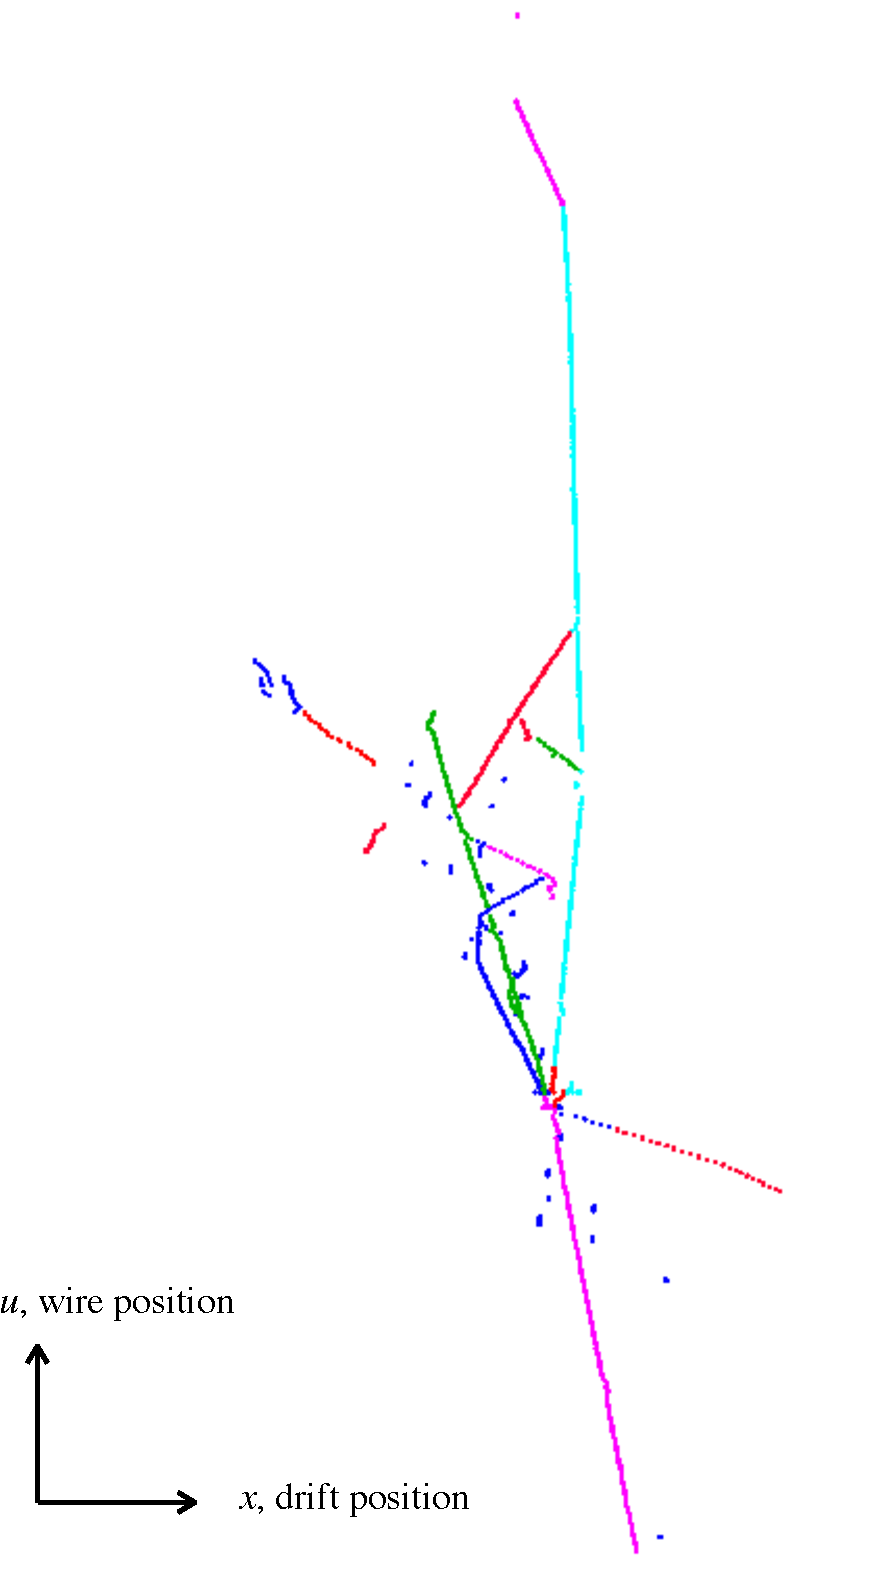
\includegraphics[width=0.3\textwidth]{Figures/EventDisplays/MC/ReconstructionU.pdf}
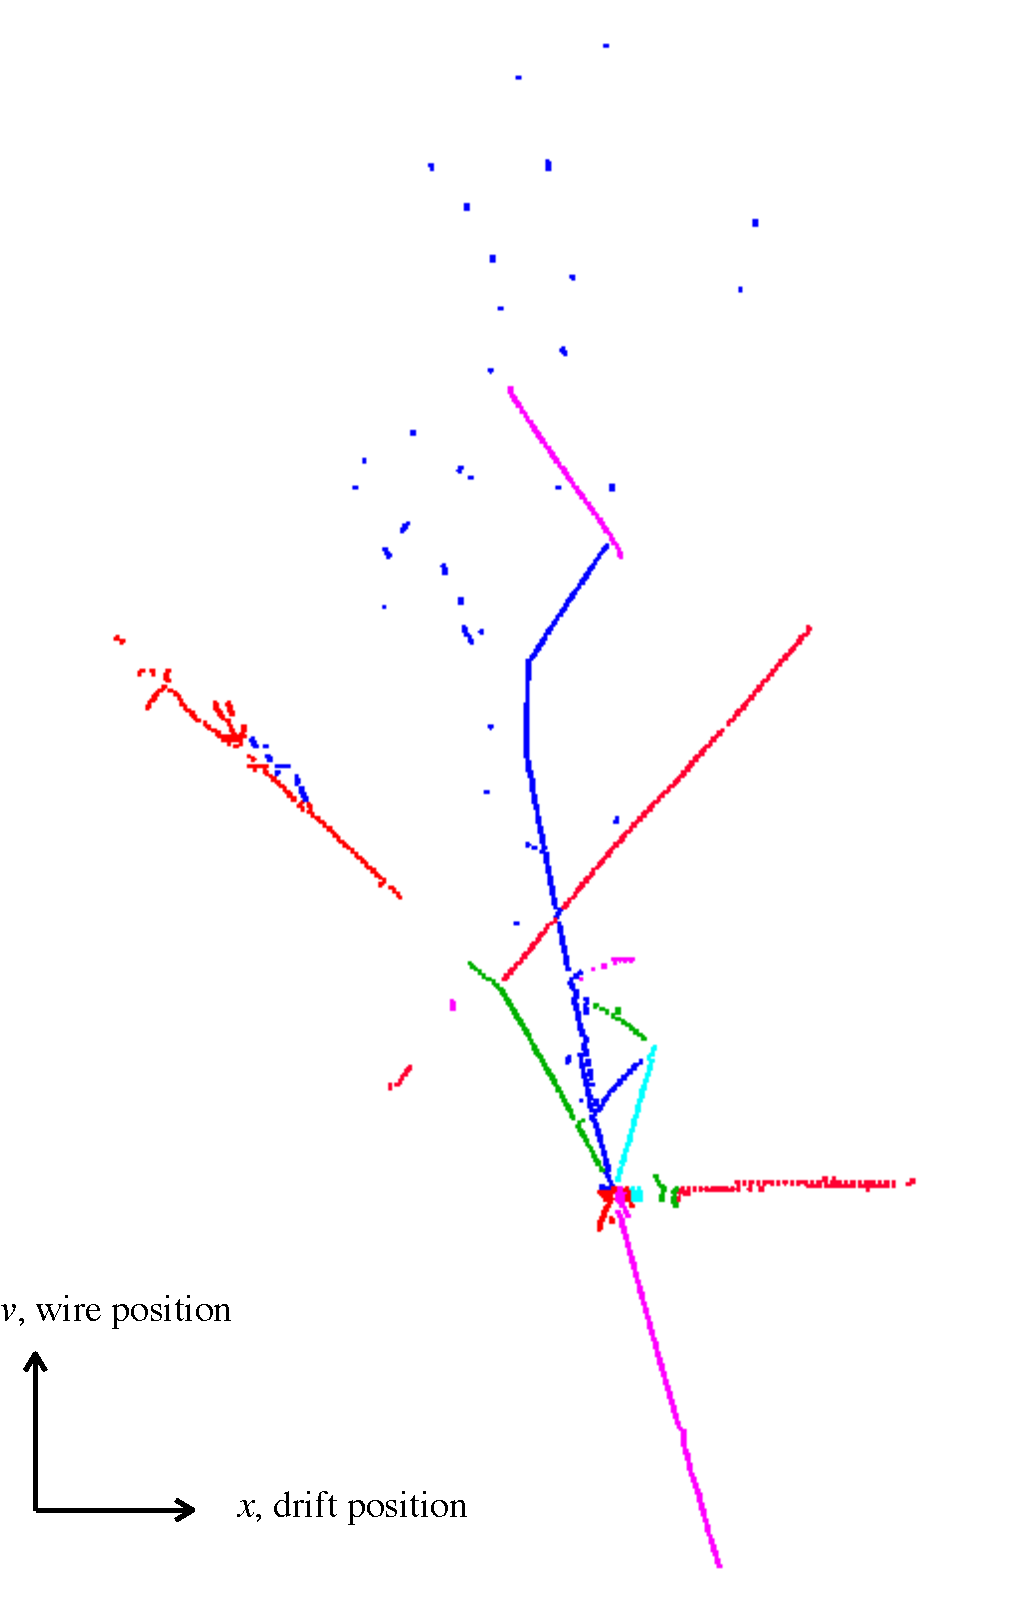
\includegraphics[width=0.3\textwidth]{Figures/EventDisplays/MC/ReconstructionV.pdf}
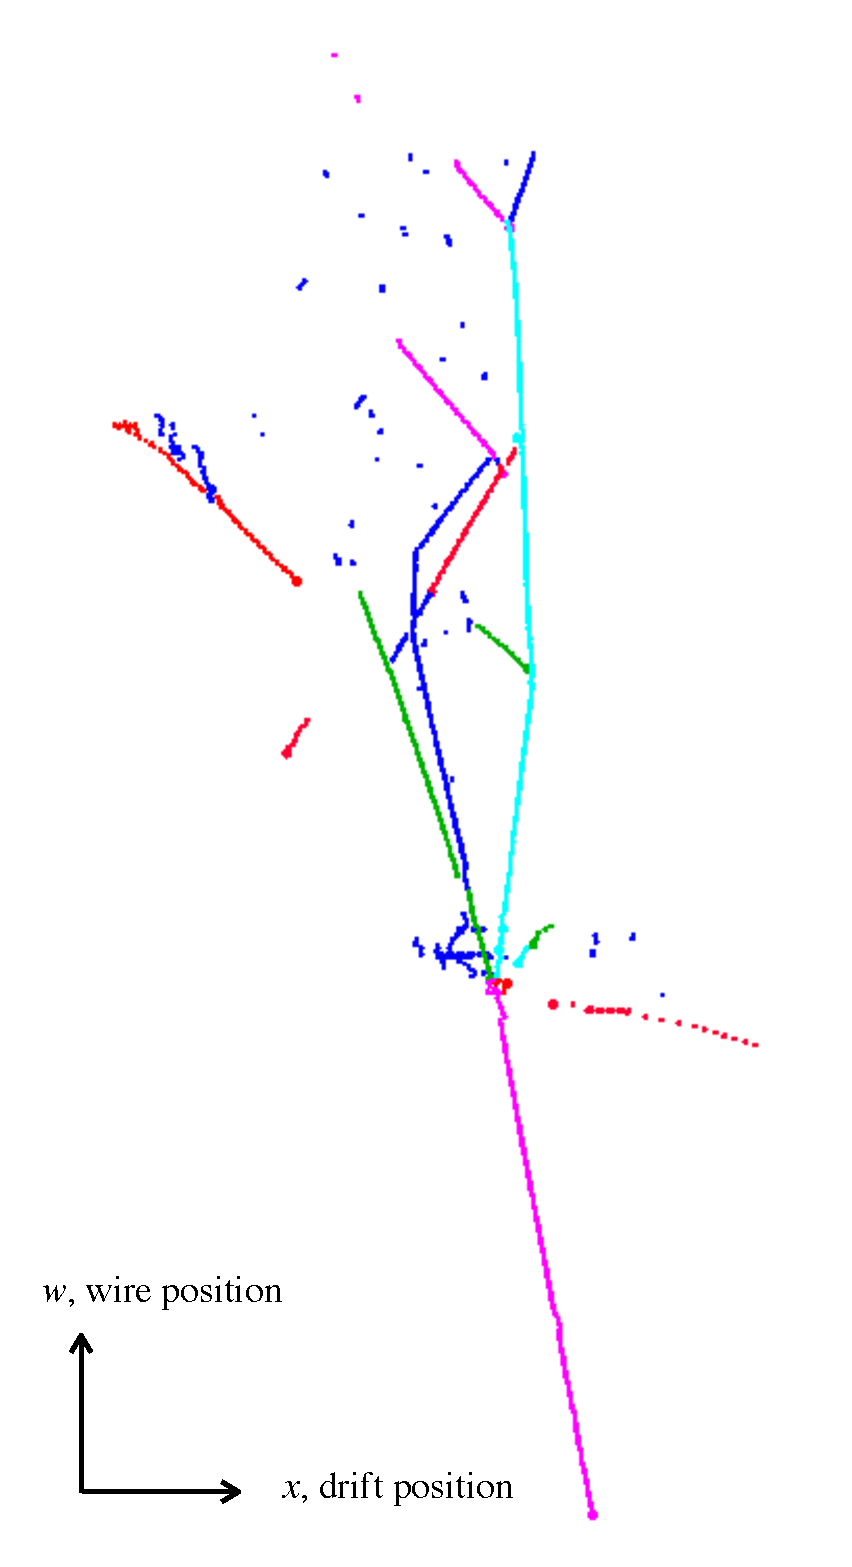
\includegraphics[width=0.3\textwidth]{Figures/EventDisplays/MC/ReconstructionW.pdf} \\
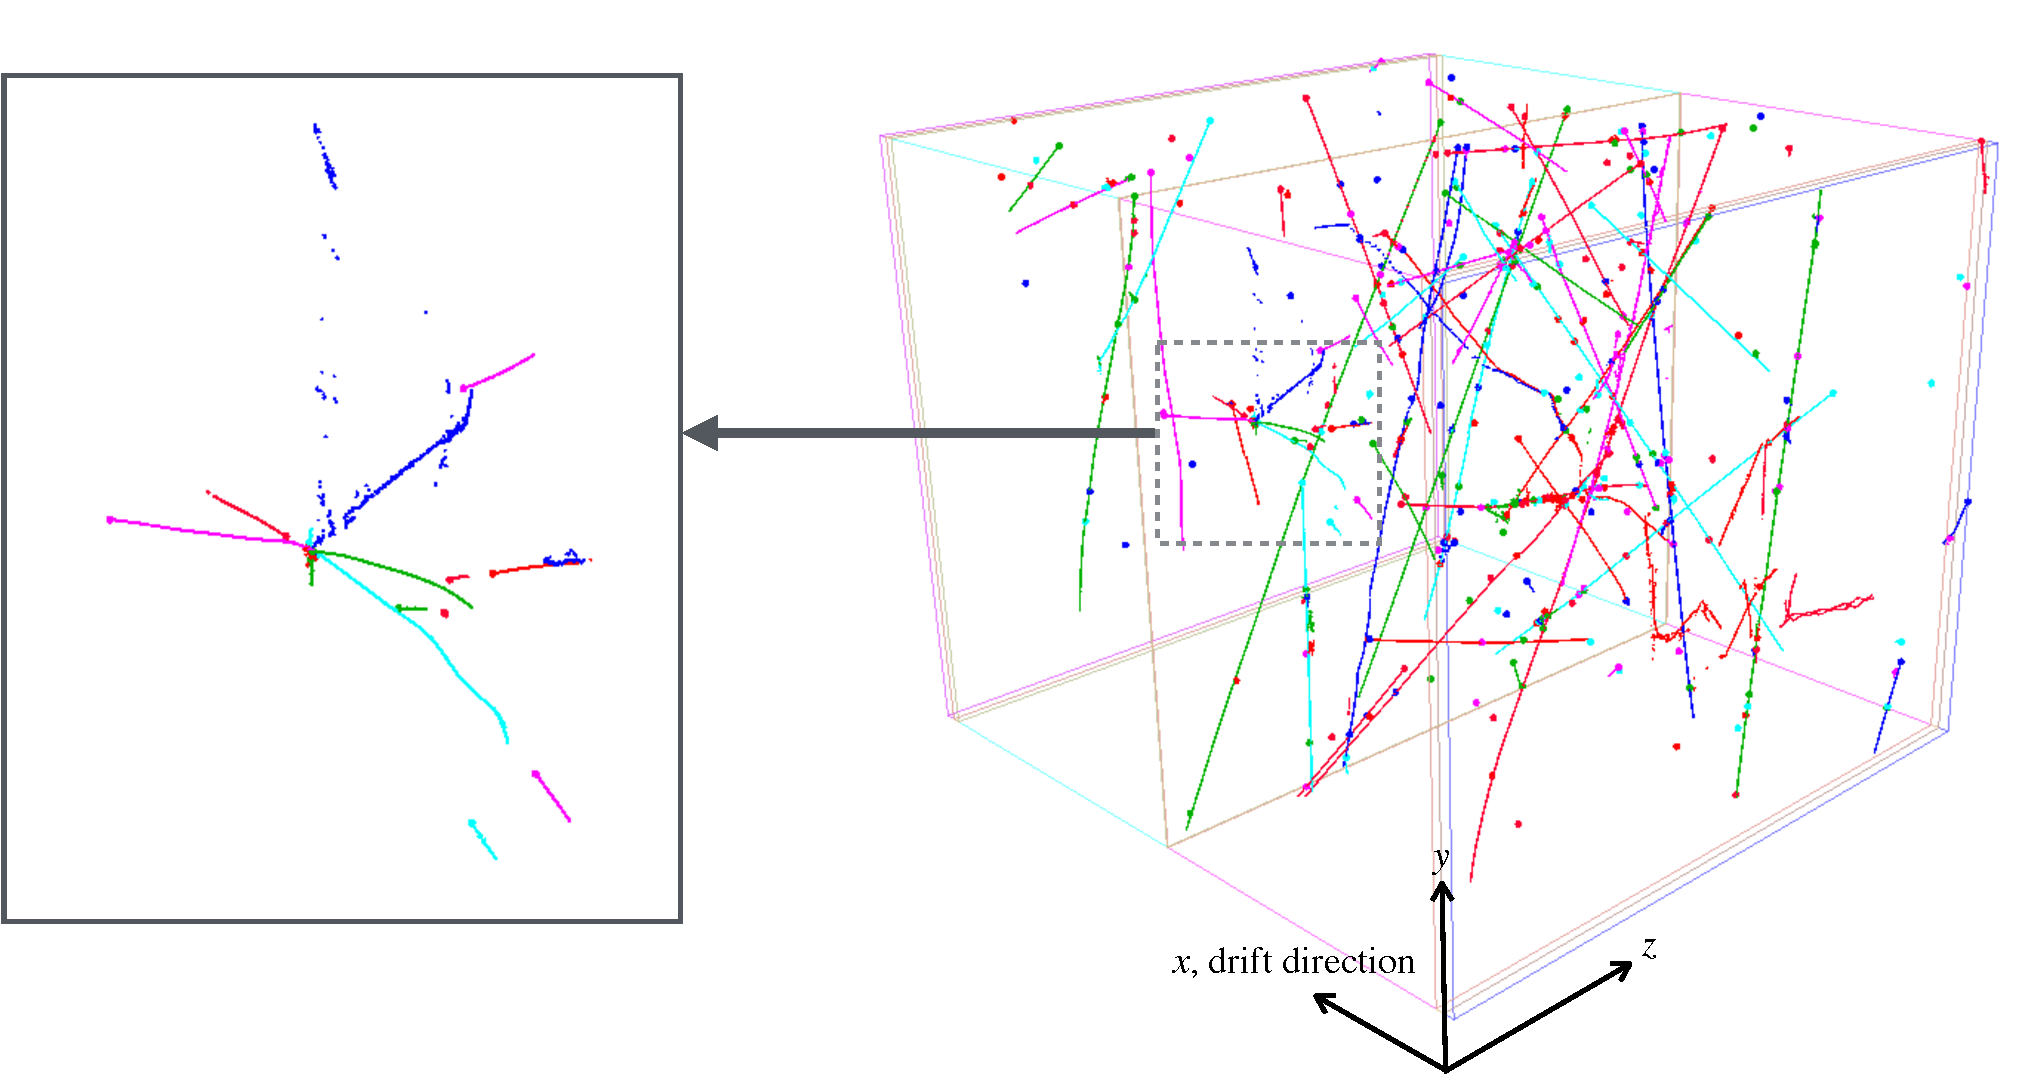
\includegraphics[width=0.75\textwidth]{Figures/EventDisplays/MC/Reconstruction.pdf} 
\caption{Please write your figure caption here}
\label{fig:1a}
\end{figure}

\begin{figure}
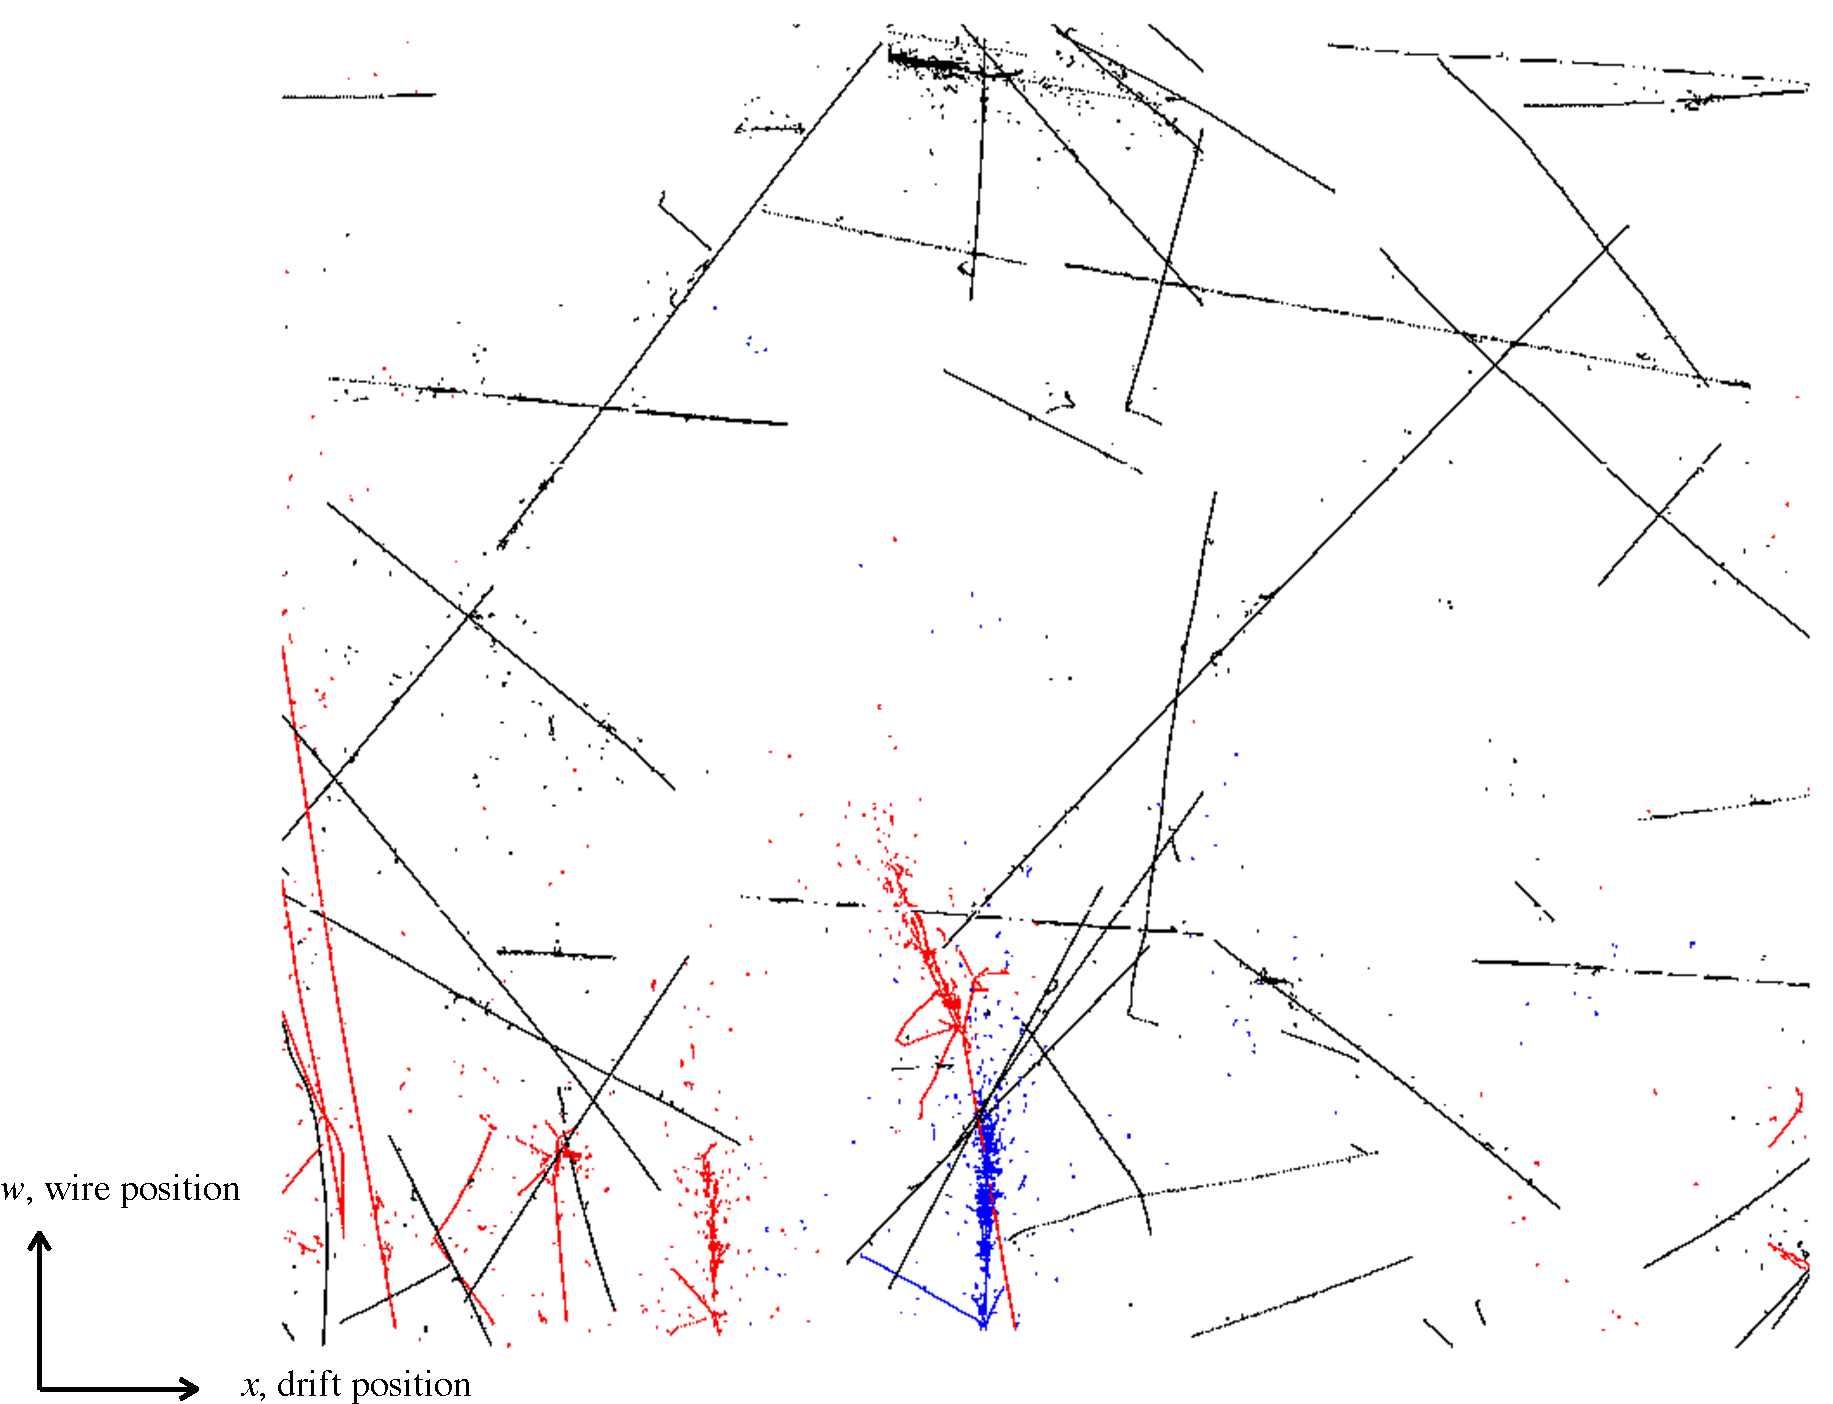
\includegraphics[width=0.75\textwidth]{Figures/EventDisplays/MC/EventComposition.pdf} 
\caption{Please write your figure caption here}
\label{fig:1b}
\end{figure}

\subsubsection{Test Beam Metrics}

Lorem ipsum dolor sit amet, consectetur adipiscing elit. Duis consectetur neque vel urna accumsan, sed tincidunt sapien tincidunt. Aenean imperdiet vitae odio rhoncus sollicitudin. Praesent nec vehicula ante. Cras aliquam hendrerit lectus, nec rutrum urna tempor a. Aliquam sit amet mattis nisl. Nam molestie a elit consectetur auctor. Lorem ipsum dolor sit amet, consectetur adipiscing elit. Nam ac magna id turpis euismod accumsan.

\begin{figure}
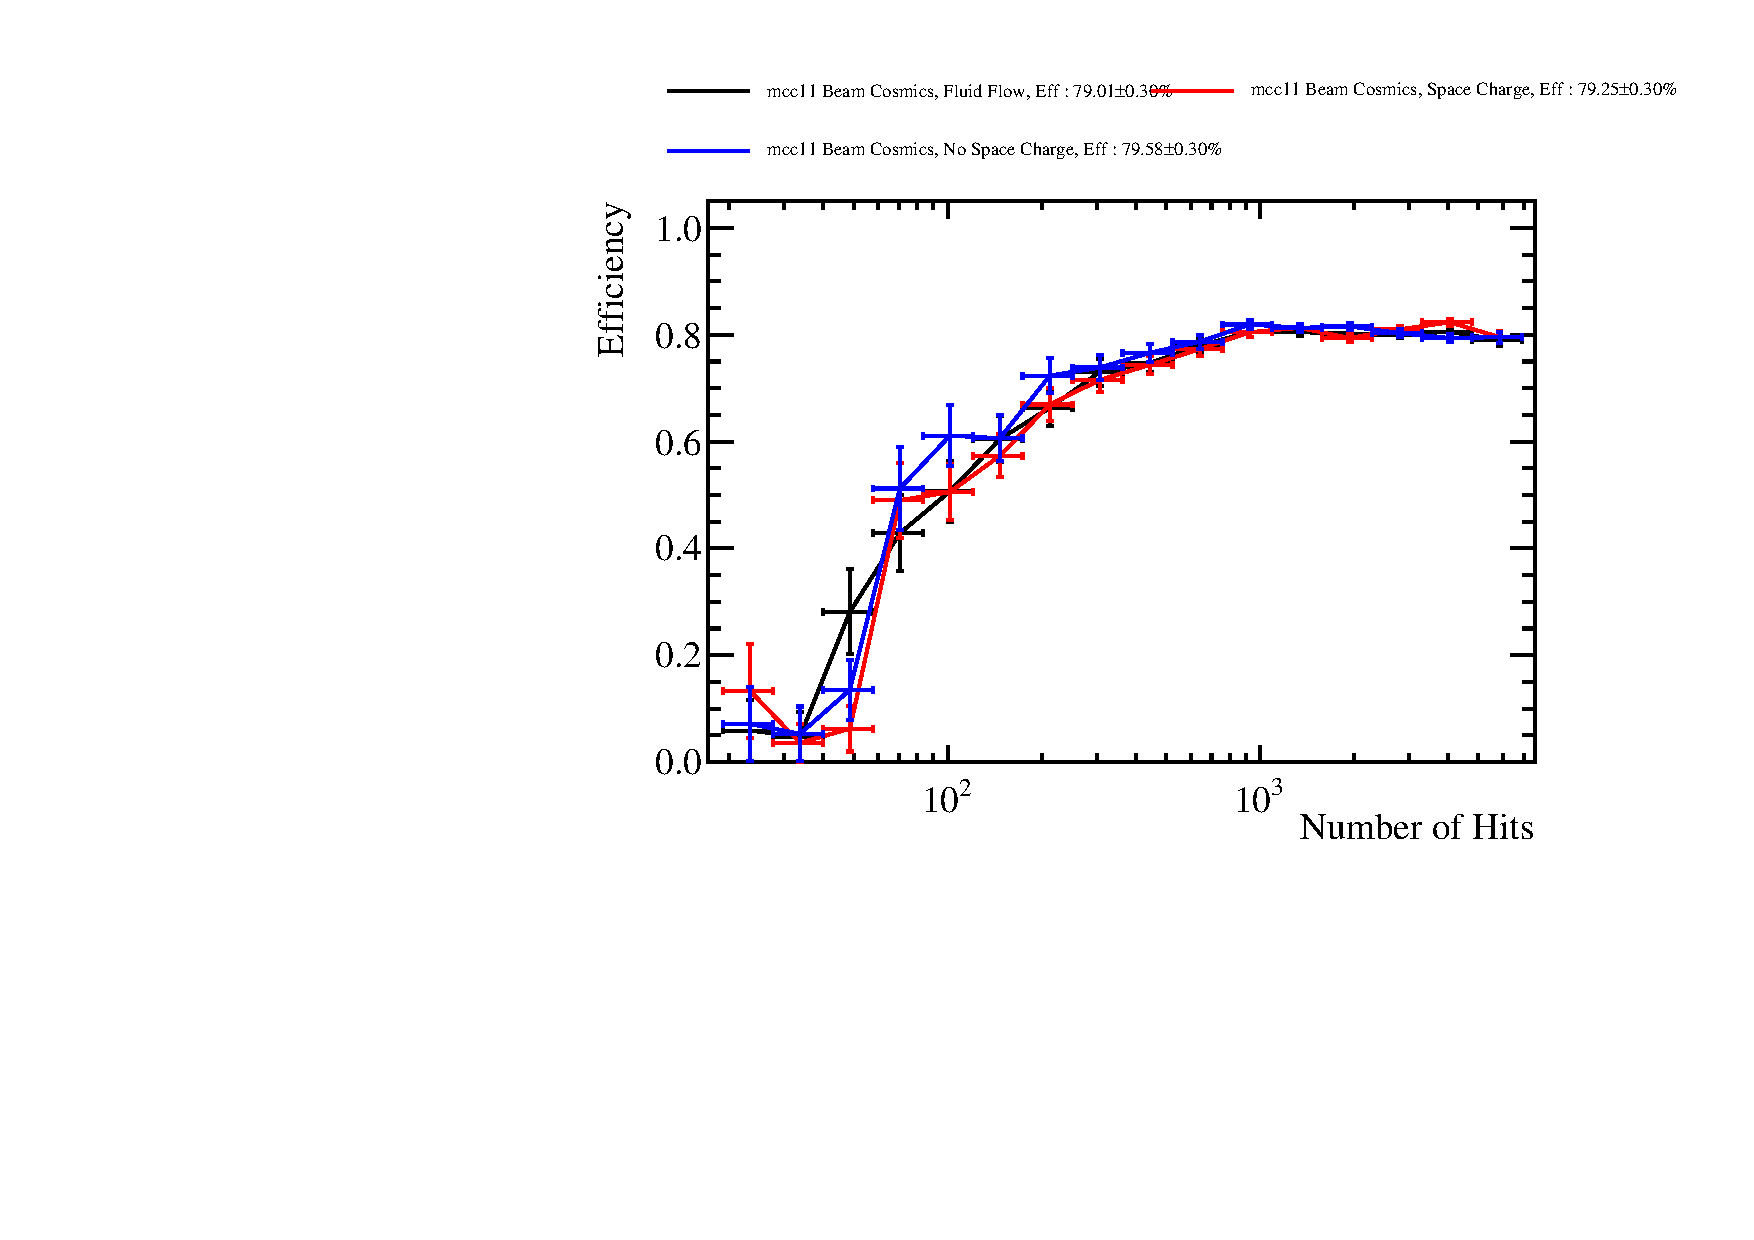
\includegraphics[width=0.5\textwidth]{Figures/Metrics/MC/Beam/BeamParticleEfficiencyBreakdownVsNHits.pdf}
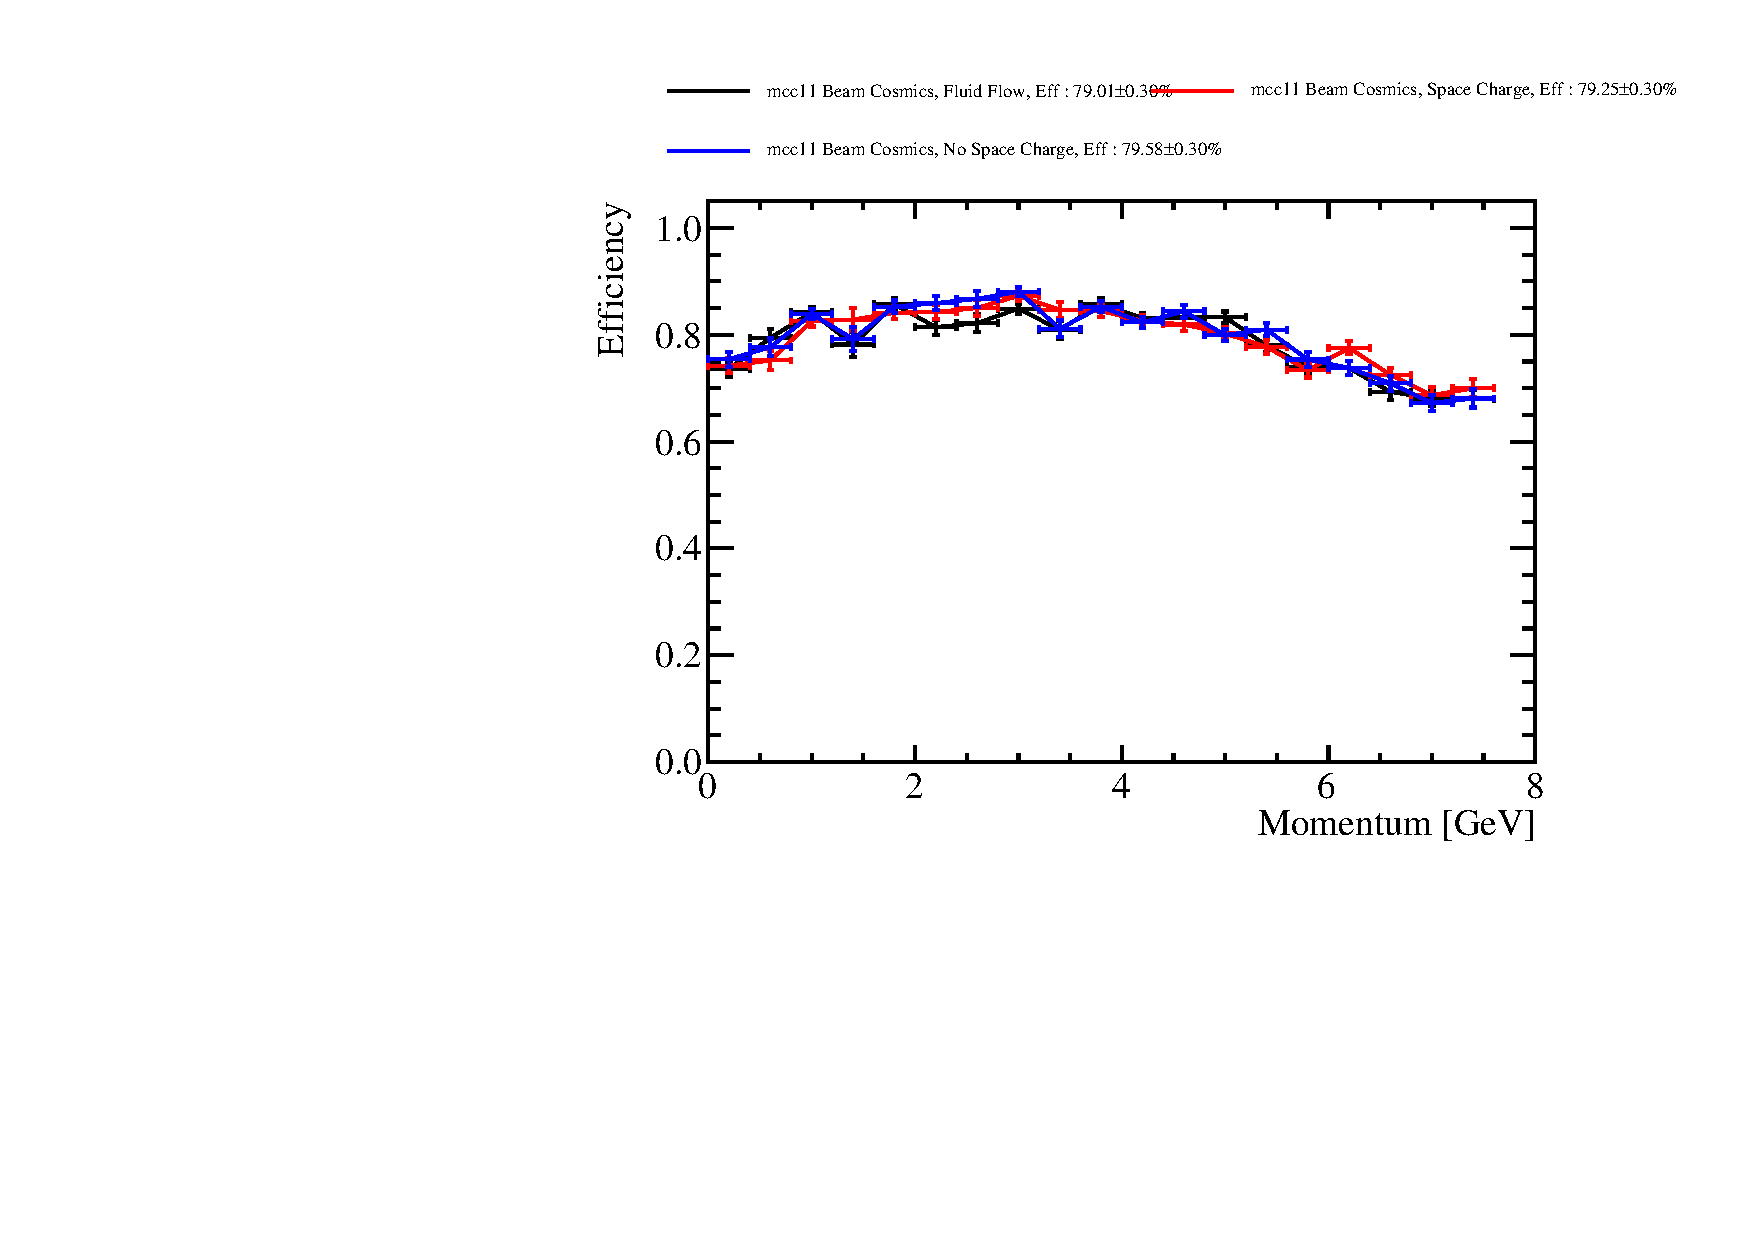
\includegraphics[width=0.5\textwidth]{Figures/Metrics/MC/Beam/BeamParticleEfficiencyBreakdownVsMomentum.pdf}
\caption{The test beam particle reconstruction efficiency as a function of the number of hits in the test beam particle and the test beam particle momentum in MC.}
\label{fig:1}
\end{figure}

\begin{table}
\caption{The reconstruction efficiency for the test beam particle in MC as a function of beam momenta.}
\label{tab:1} 
\begin{tabular}{cc}
\hline\noalign{\smallskip}
Beam Momenta [GeV] & Reconstructed Efficiency  \\
\noalign{\smallskip}\hline\noalign{\smallskip}
1 & 87.5$\pm$0.8 \\
2 & 91.0$\pm$0.7 \\
3 & 92.7$\pm$0.6 \\
4 & 89.8$\pm$0.5 \\
5 & 89.0$\pm$0.5 \\
6 & 82.1$\pm$0.7 \\
7 & 75.4$\pm$0.7 \\
\noalign{\smallskip}\hline
\end{tabular}
\end{table}

\begin{figure}
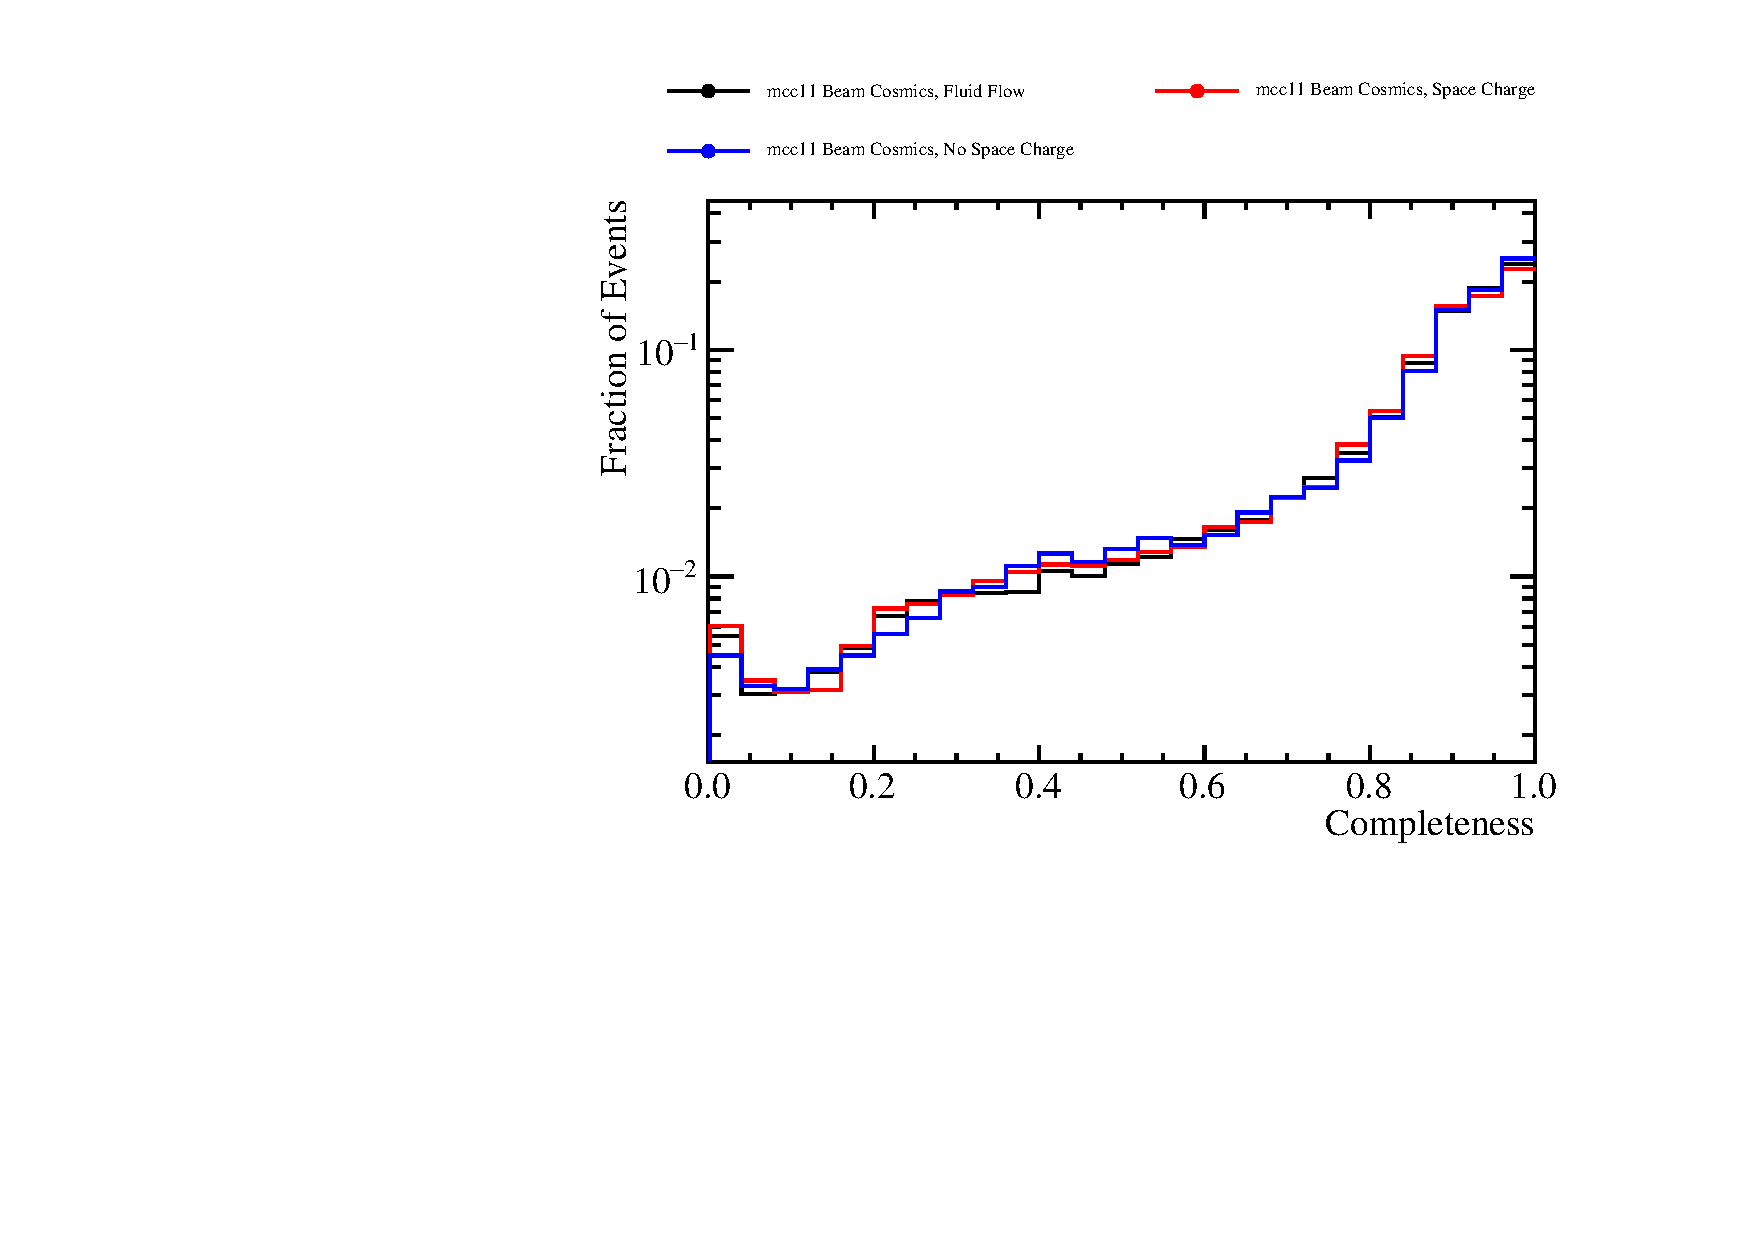
\includegraphics[width=0.5\textwidth]{Figures/Metrics/MC/Beam/BeamParticleCompleteness.pdf}
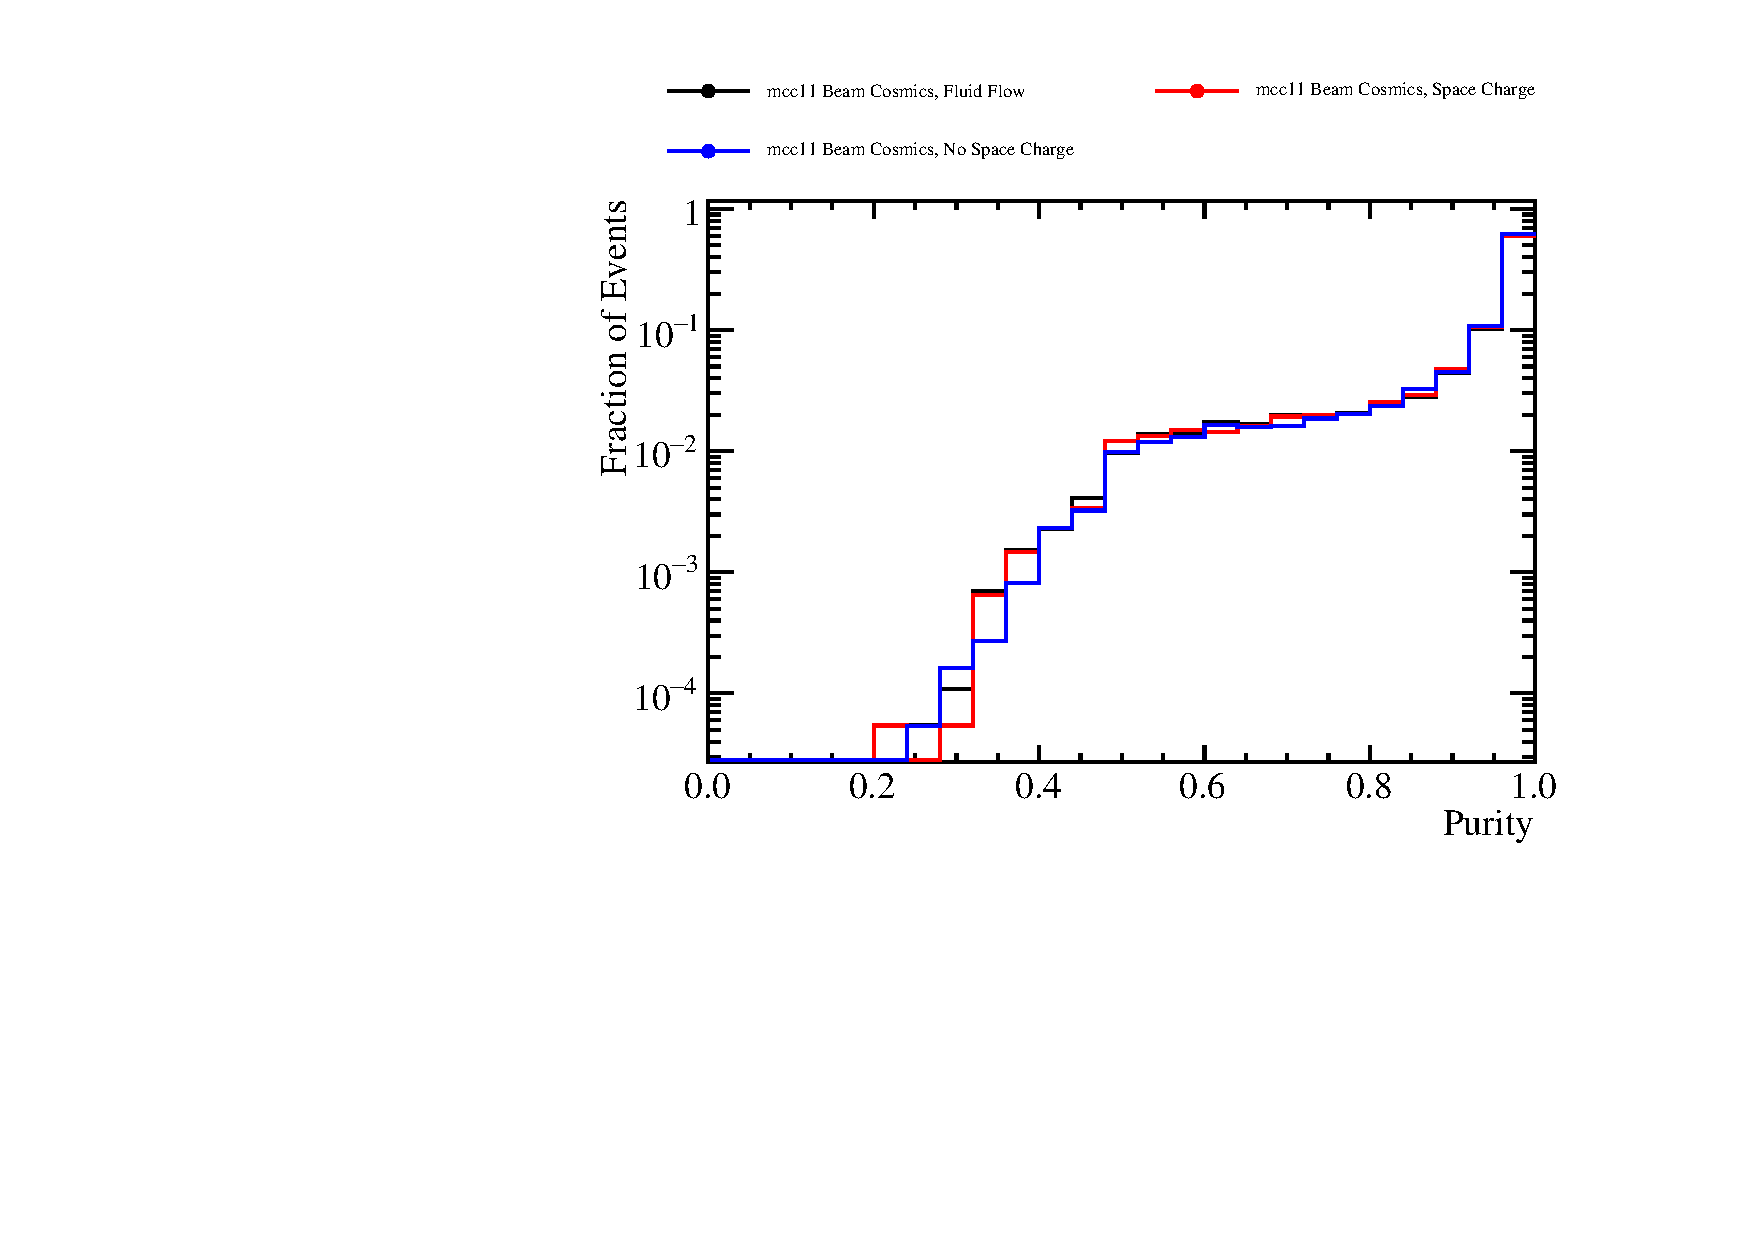
\includegraphics[width=0.5\textwidth]{Figures/Metrics/MC/Beam/BeamParticlePurity.pdf}
\caption{The purity and completeness of reconstructed test beam particles in MC.}
\label{fig:2}
\end{figure}

\subsubsection{Cosmic Ray Metrics}

Lorem ipsum dolor sit amet, consectetur adipiscing elit. Duis consectetur neque vel urna accumsan, sed tincidunt sapien tincidunt. Aenean imperdiet vitae odio rhoncus sollicitudin. Praesent nec vehicula ante. Cras aliquam hendrerit lectus, nec rutrum urna tempor a. Aliquam sit amet mattis nisl. Nam molestie a elit consectetur auctor. Lorem ipsum dolor sit amet, consectetur adipiscing elit. Nam ac magna id turpis euismod accumsan.

\begin{figure}
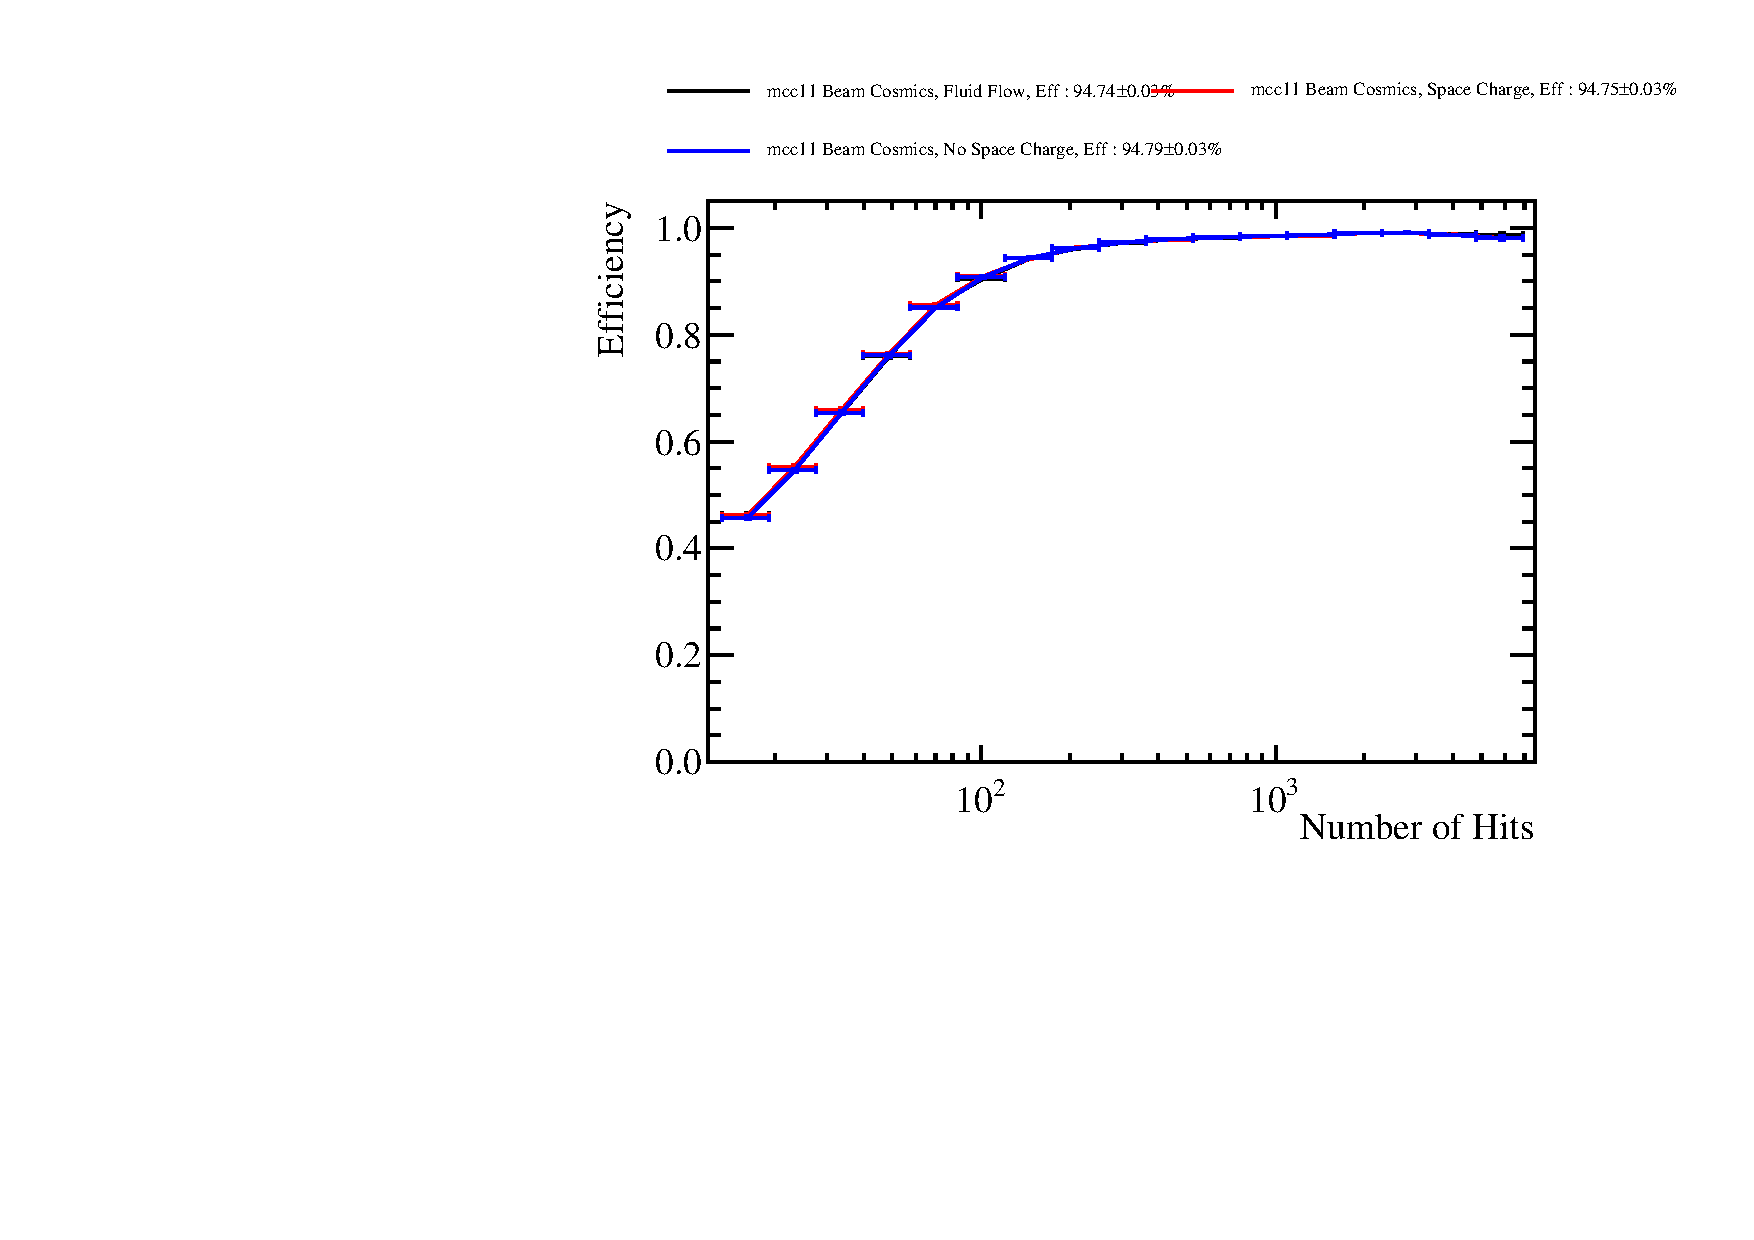
\includegraphics[width=0.75\textwidth]{Figures/Metrics/MC/Cosmics/CosmicRayEfficiencyVsNHits.pdf}
\caption{The reconstruction efficiency for cosmic rays in MC as a function of number of hits.}
\label{fig:3}
\end{figure}

\begin{figure}
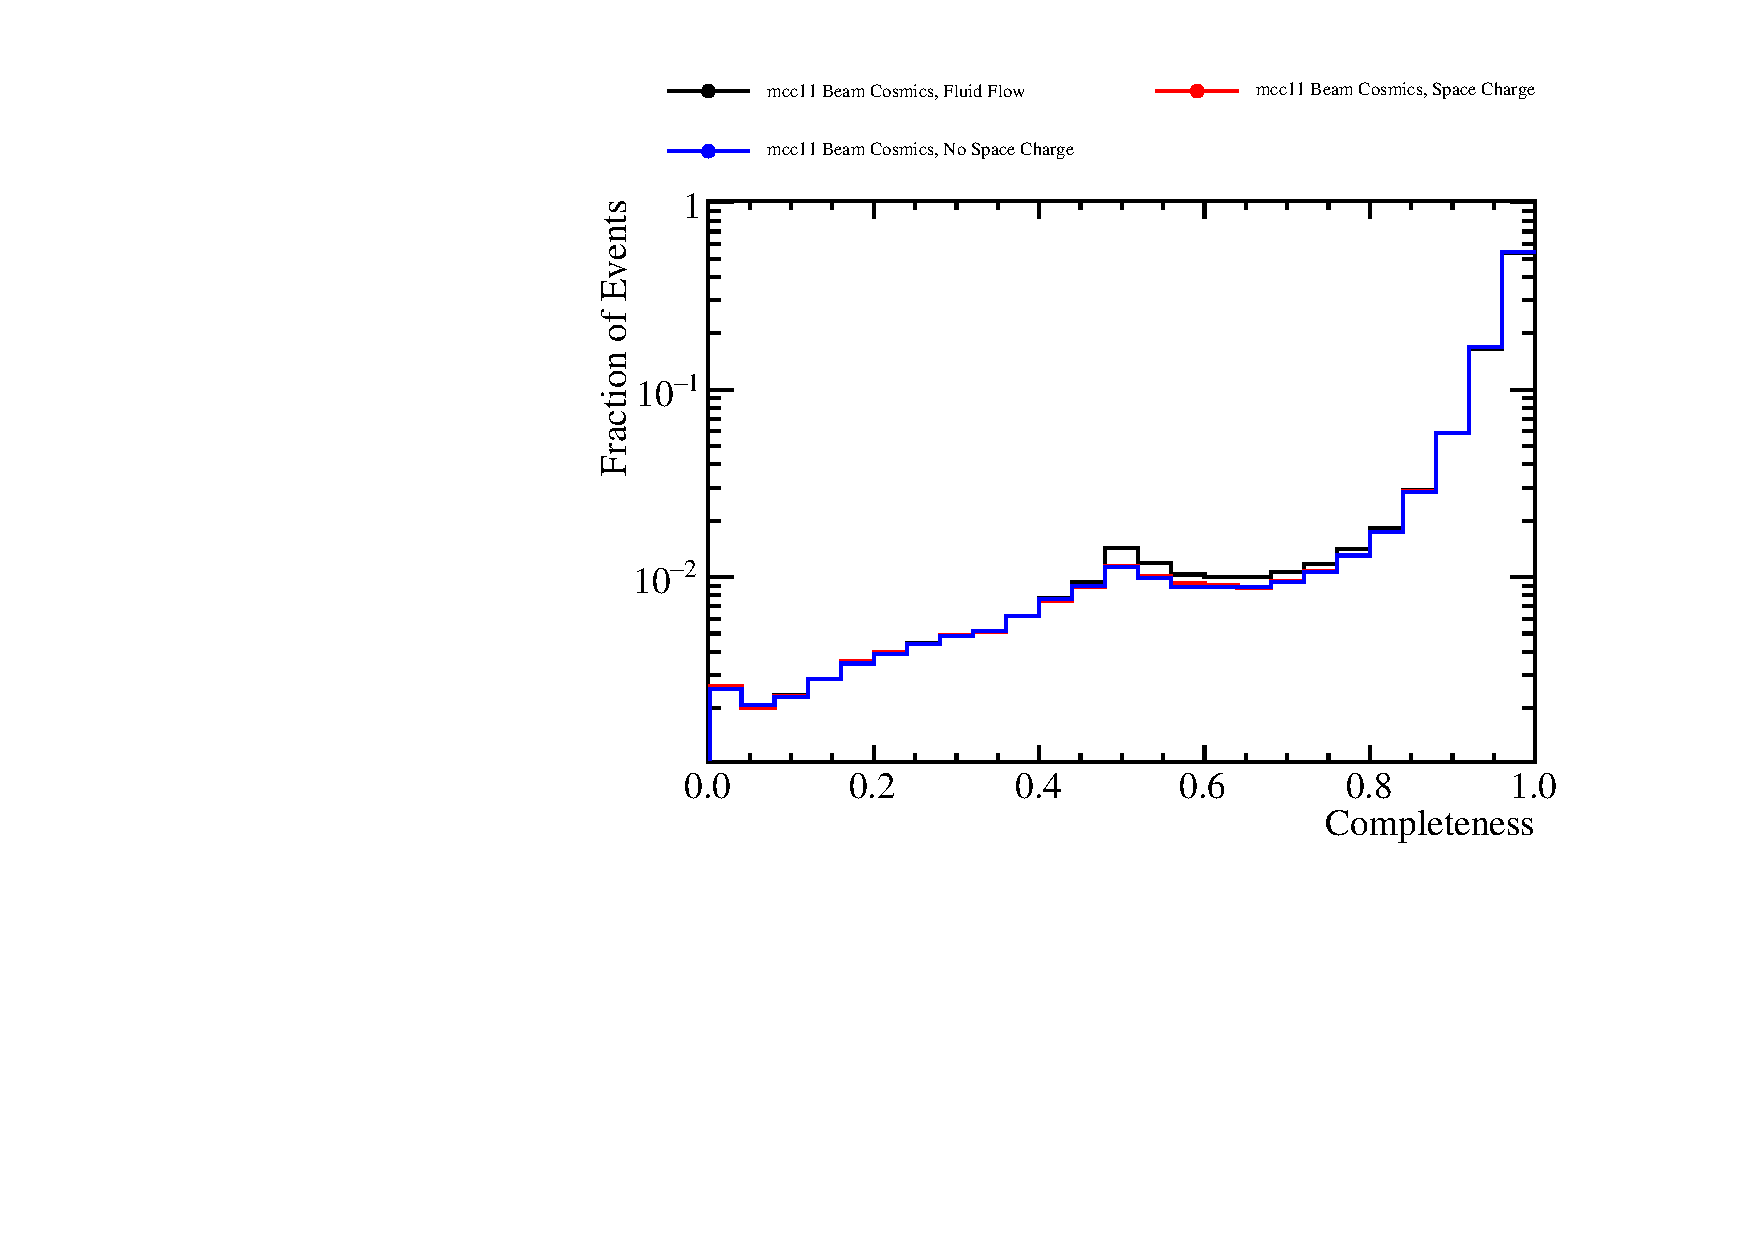
\includegraphics[width=0.5\textwidth]{Figures/Metrics/MC/Cosmics/CosmicRayCompleteness.pdf}
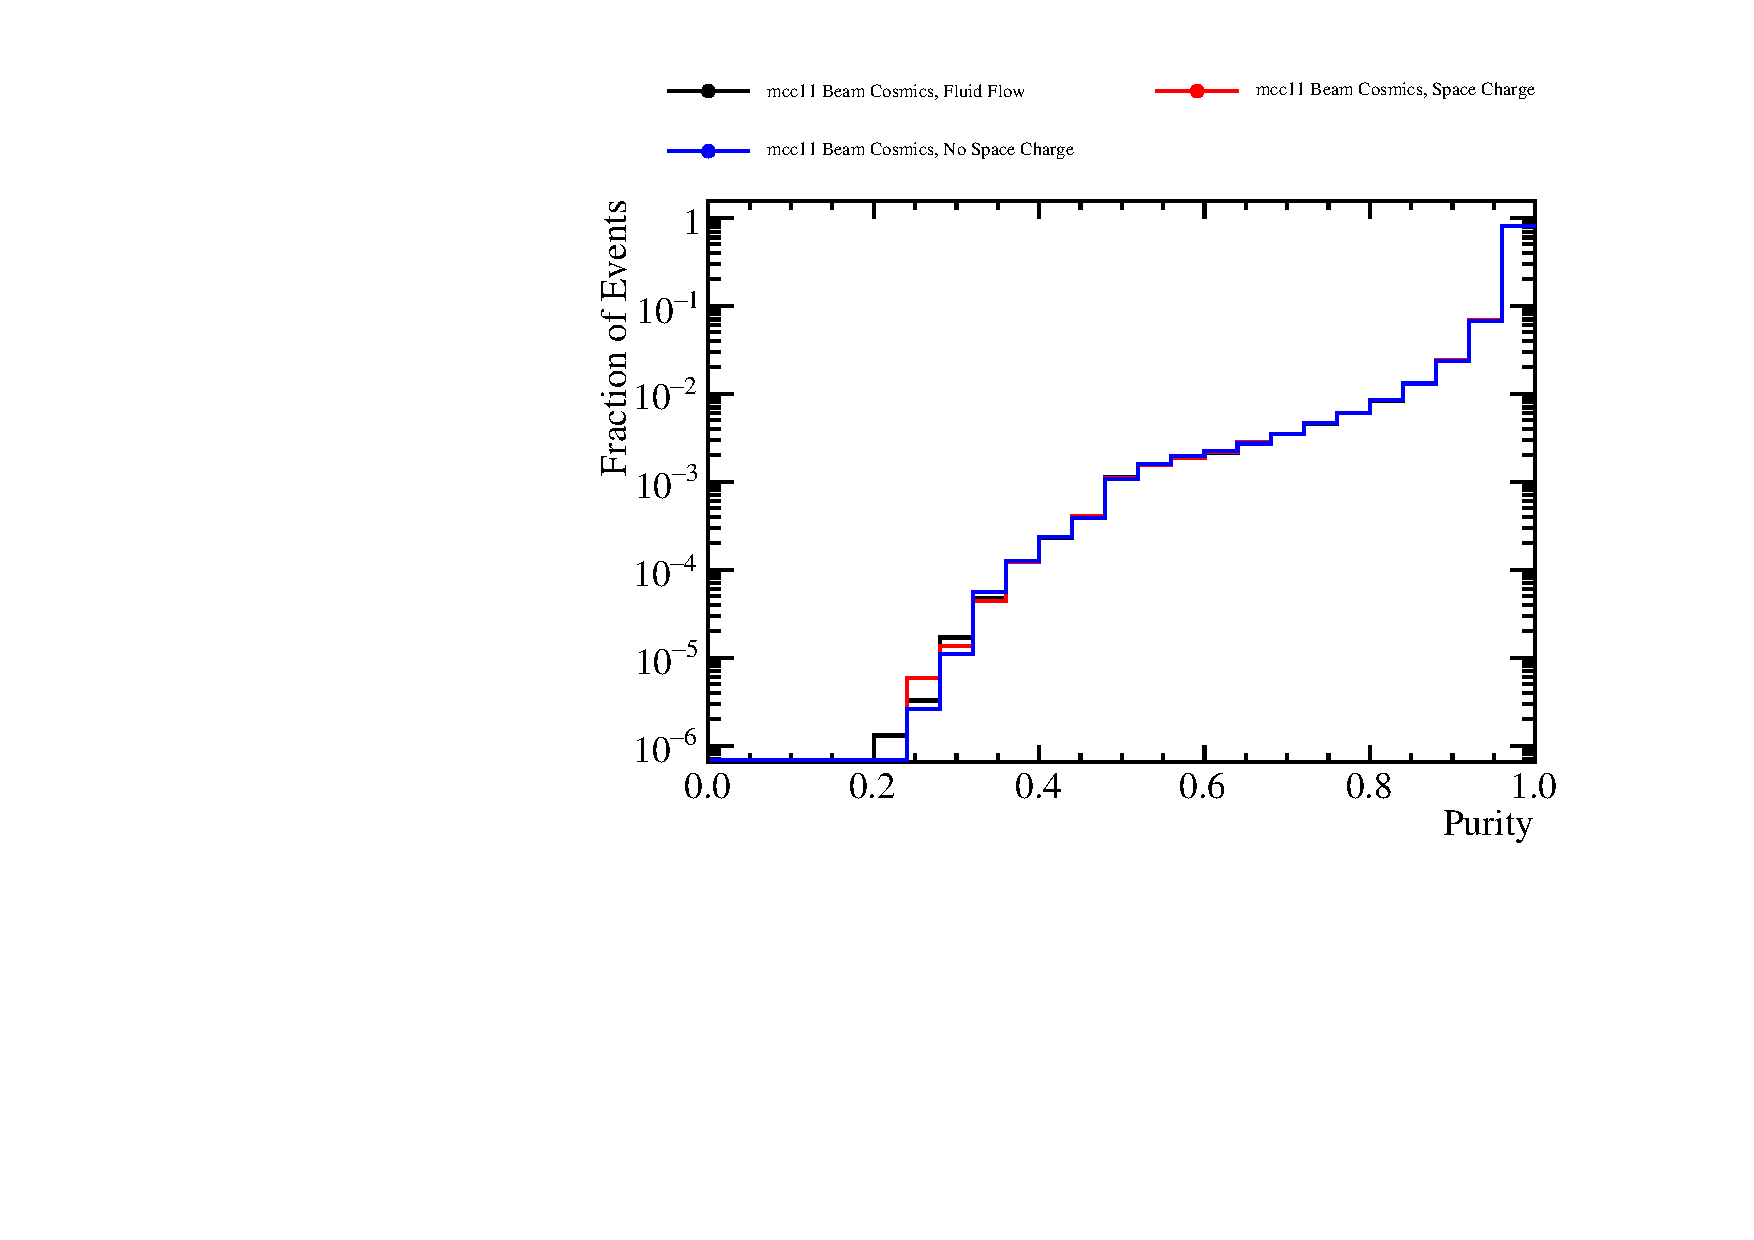
\includegraphics[width=0.5\textwidth]{Figures/Metrics/MC/Cosmics/CosmicRayPurity.pdf}
\caption{The purity and completeness of reconstructed cosmic ray particles in MC.}
\label{fig:4}
\end{figure}

\begin{figure}
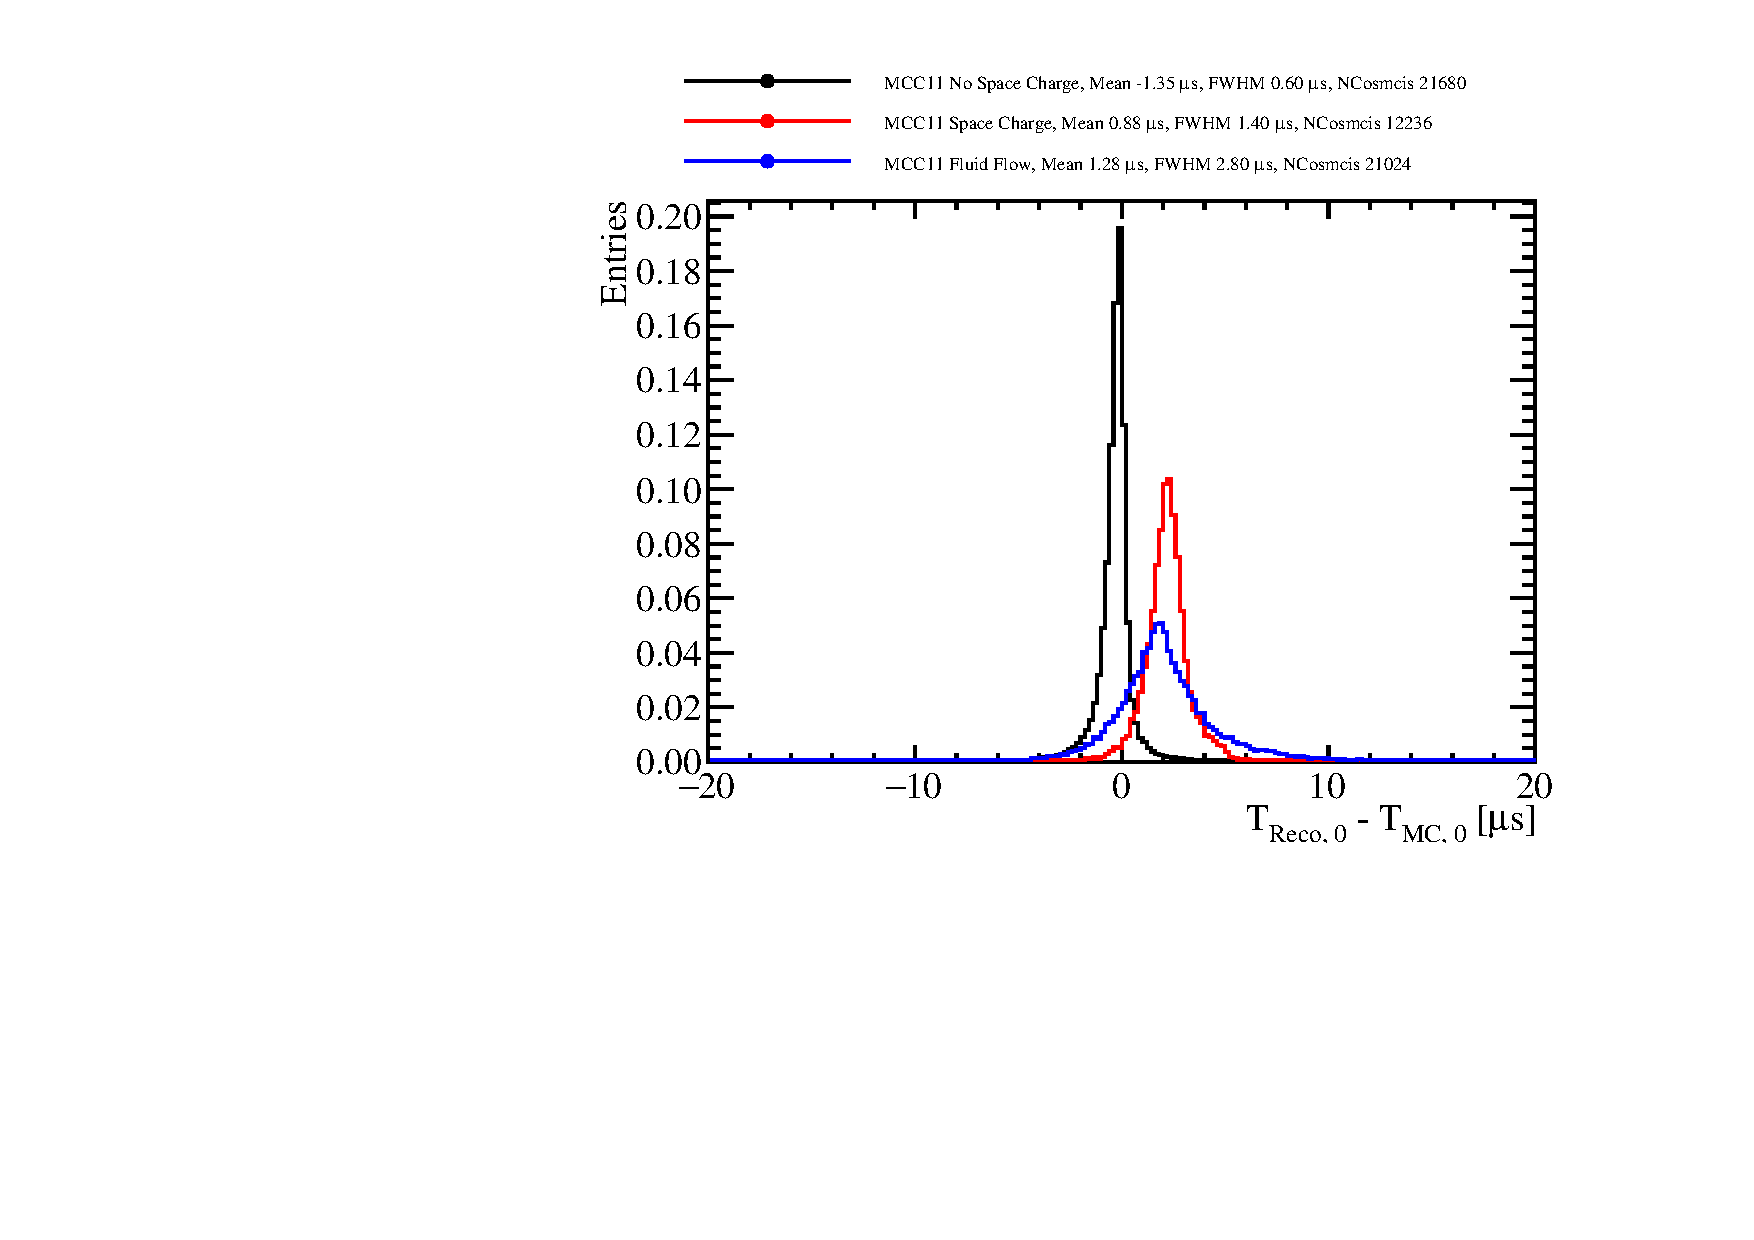
\includegraphics[width=1.0\textwidth]{Figures/Metrics/MC/Cosmics/CosmicRayT0Resolustion.pdf}
\caption{The resolution on the reconstructed $T_{0}$ for cosmic rays in MC.}
\label{fig:5}
\end{figure}

\begin{figure}
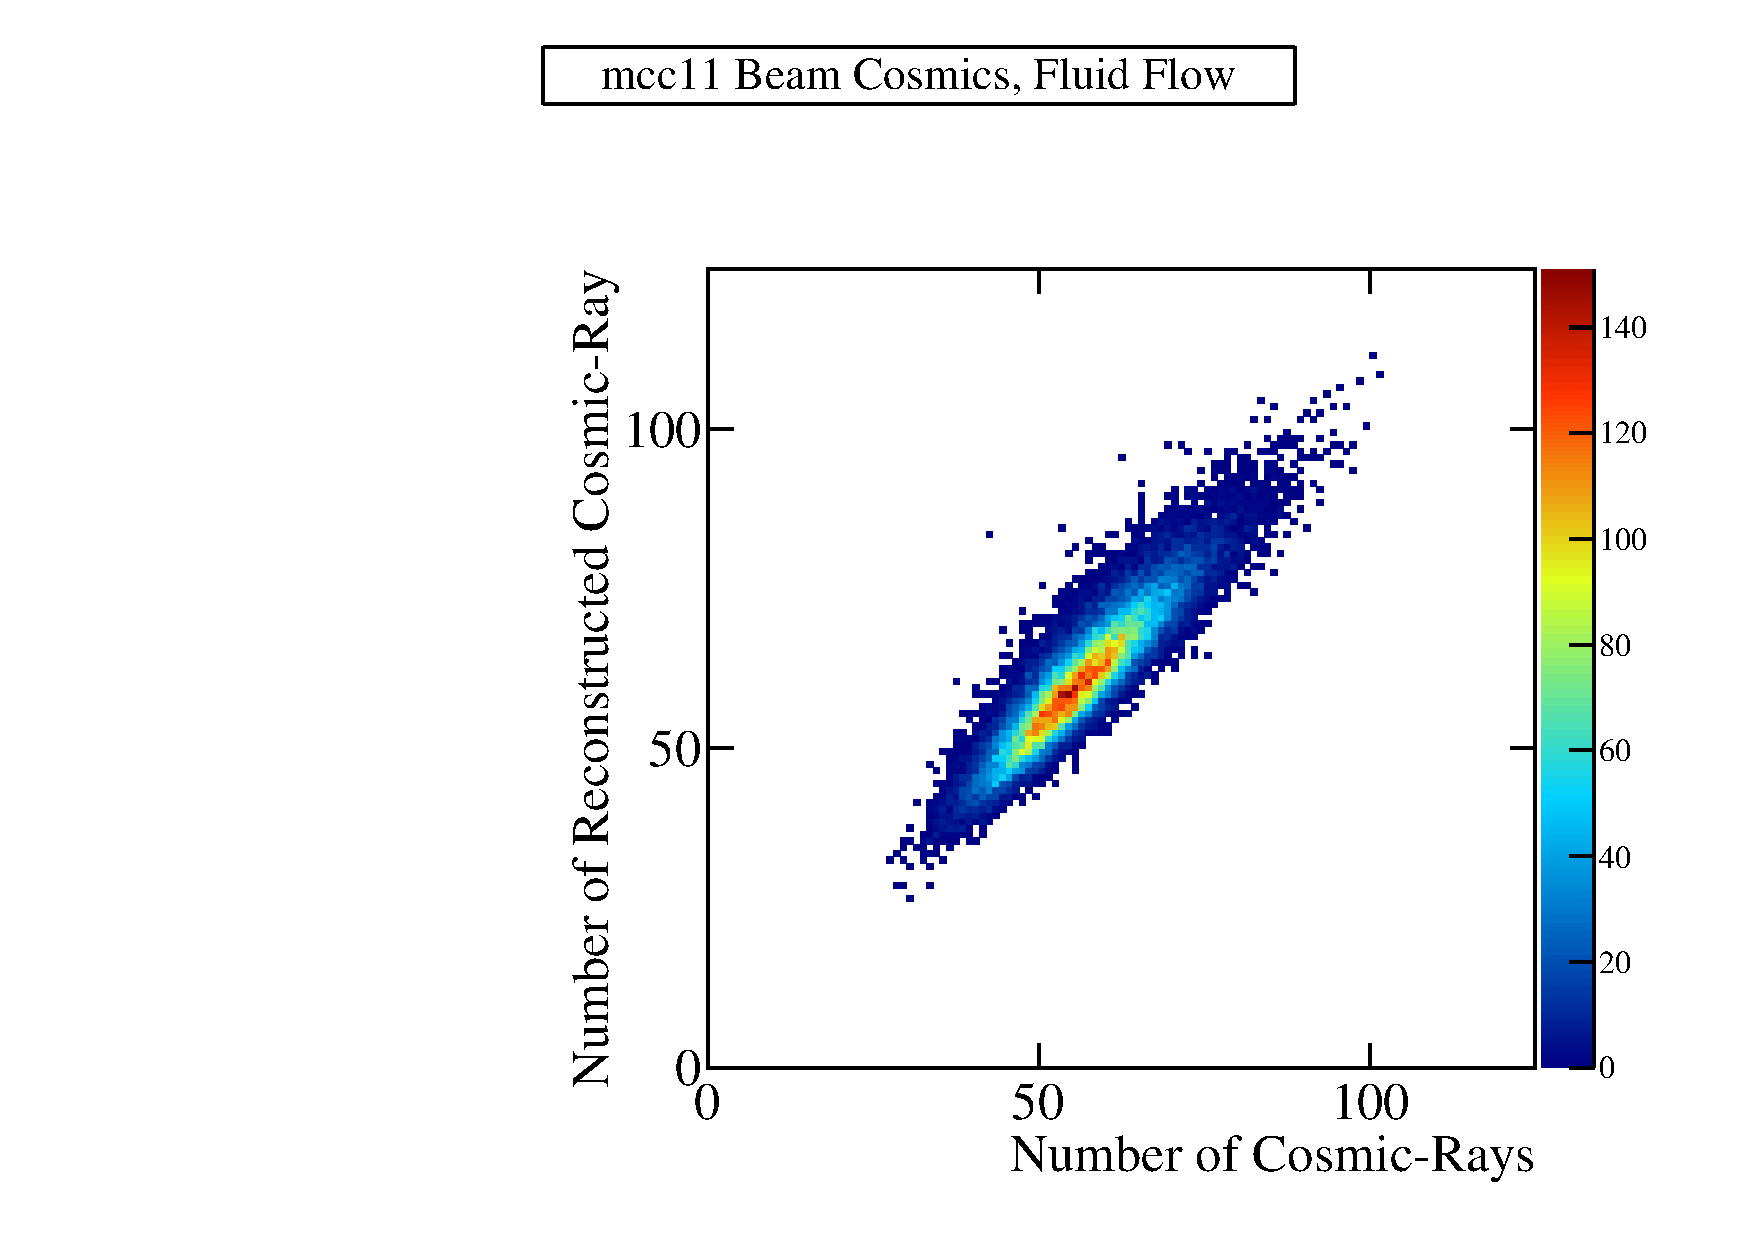
\includegraphics[width=0.5\textwidth]{Figures/Metrics/MC/Cosmics/CRMatchesCosmicRayEvent.pdf}
\caption{The number of reconstructed cosmic rays per event as a function of the true number of reconstructable cosmic rays in the event.}
\label{fig:6}
\end{figure}

\subsection{Data}

Lorem ipsum dolor sit amet, consectetur adipiscing elit. Duis consectetur neque vel urna accumsan, sed tincidunt sapien tincidunt. Aenean imperdiet vitae odio rhoncus sollicitudin. Praesent nec vehicula ante. Cras aliquam hendrerit lectus, nec rutrum urna tempor a. Aliquam sit amet mattis nisl. Nam molestie a elit consectetur auctor. Lorem ipsum dolor sit amet, consectetur adipiscing elit. Nam ac magna id turpis euismod accumsan.

Aliquam gravida urna a arcu euismod, eget ultricies enim placerat. Vestibulum ultrices ultricies eleifend. Proin vestibulum risus eu ultrices condimentum. Interdum et malesuada fames ac ante ipsum primis in faucibus. Aliquam id urna in dui tristique feugiat. Nullam in dui diam. Etiam sit amet eros vel mi egestas scelerisque sed nec nibh. Vivamus imperdiet risus sed quam commodo vehicula. Nulla in arcu scelerisque, luctus urna ut, ullamcorper est. Fusce tristique eros in tempus egestas. Phasellus non mattis risus. Quisque sed tristique lectus. Donec porttitor commodo enim dictum facilisis.

Pellentesque consequat accumsan auctor. Vivamus efficitur urna a augue molestie lacinia. Morbi et facilisis quam. Praesent libero velit, lobortis ac posuere sit amet, pharetra non nunc. Donec porttitor malesuada tristique. Suspendisse suscipit ultrices turpis, congue mattis odio facilisis ac. Proin ornare metus a velit lacinia, non vulputate massa ultrices. Proin diam leo, tristique non lectus ut, pellentesque malesuada enim. Phasellus tortor nulla, cursus ac sapien in, tempor sollicitudin ante. Ut ac dui nec erat eleifend varius. Vestibulum placerat urna quis feugiat imperdiet.

\subsubsection{Test Beam Metrics}

Lorem ipsum dolor sit amet, consectetur adipiscing elit. Duis consectetur neque vel urna accumsan, sed tincidunt sapien tincidunt. Aenean imperdiet vitae odio rhoncus sollicitudin. Praesent nec vehicula ante. Cras aliquam hendrerit lectus, nec rutrum urna tempor a. Aliquam sit amet mattis nisl. Nam molestie a elit consectetur auctor. Lorem ipsum dolor sit amet, consectetur adipiscing elit. Nam ac magna id turpis euismod accumsan.

\begin{figure}
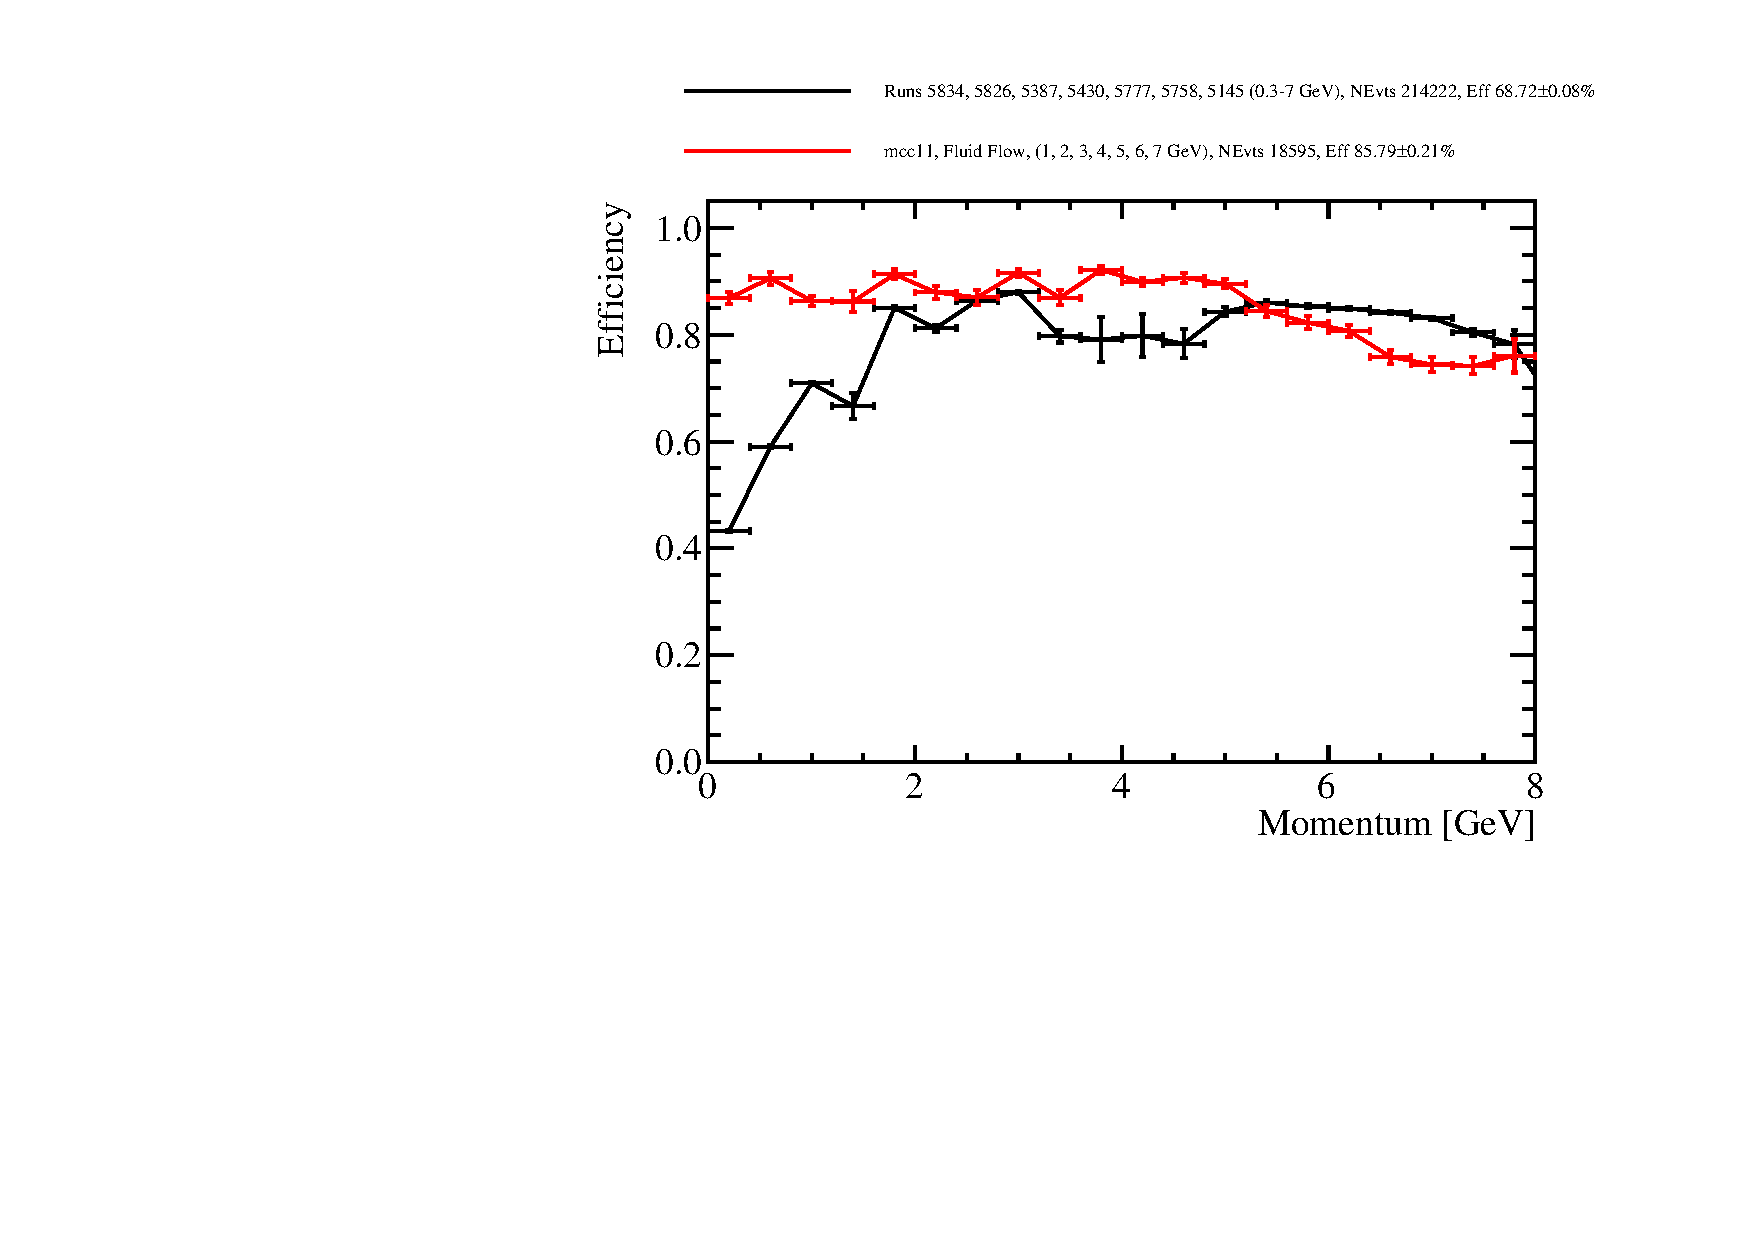
\includegraphics[width=1.0\textwidth]{Figures/Metrics/Data/Beam/BeamParticleEfficiencyVsMomentum.pdf}
\caption{The test beam particle reconstruction efficiency as a function of the number of hits in the test beam particle and the test beam particle momentum.}
\label{fig:7}
\end{figure}

\begin{table}
\caption{The reconstruction efficiency for the test beam particle in data as a function of beam momenta.}
\label{tab:1} 
\begin{tabular}{cc}
\hline\noalign{\smallskip}
Beam Momenta [GeV] & Reconstructed Efficiency  \\
\noalign{\smallskip}\hline\noalign{\smallskip}
0.3 & 43.2$\pm$0.3 \\
0.5 & 55.4$\pm$0.2 \\
1 & 70.6$\pm$0.3 \\
2 & 84.2$\pm$0.3 \\
3 & 86.8$\pm$0.2 \\
6 & 85.2$\pm$0.2 \\
7 & 83.7$\pm$0.2 \\
\noalign{\smallskip}\hline
\end{tabular}
\end{table}

\begin{figure}
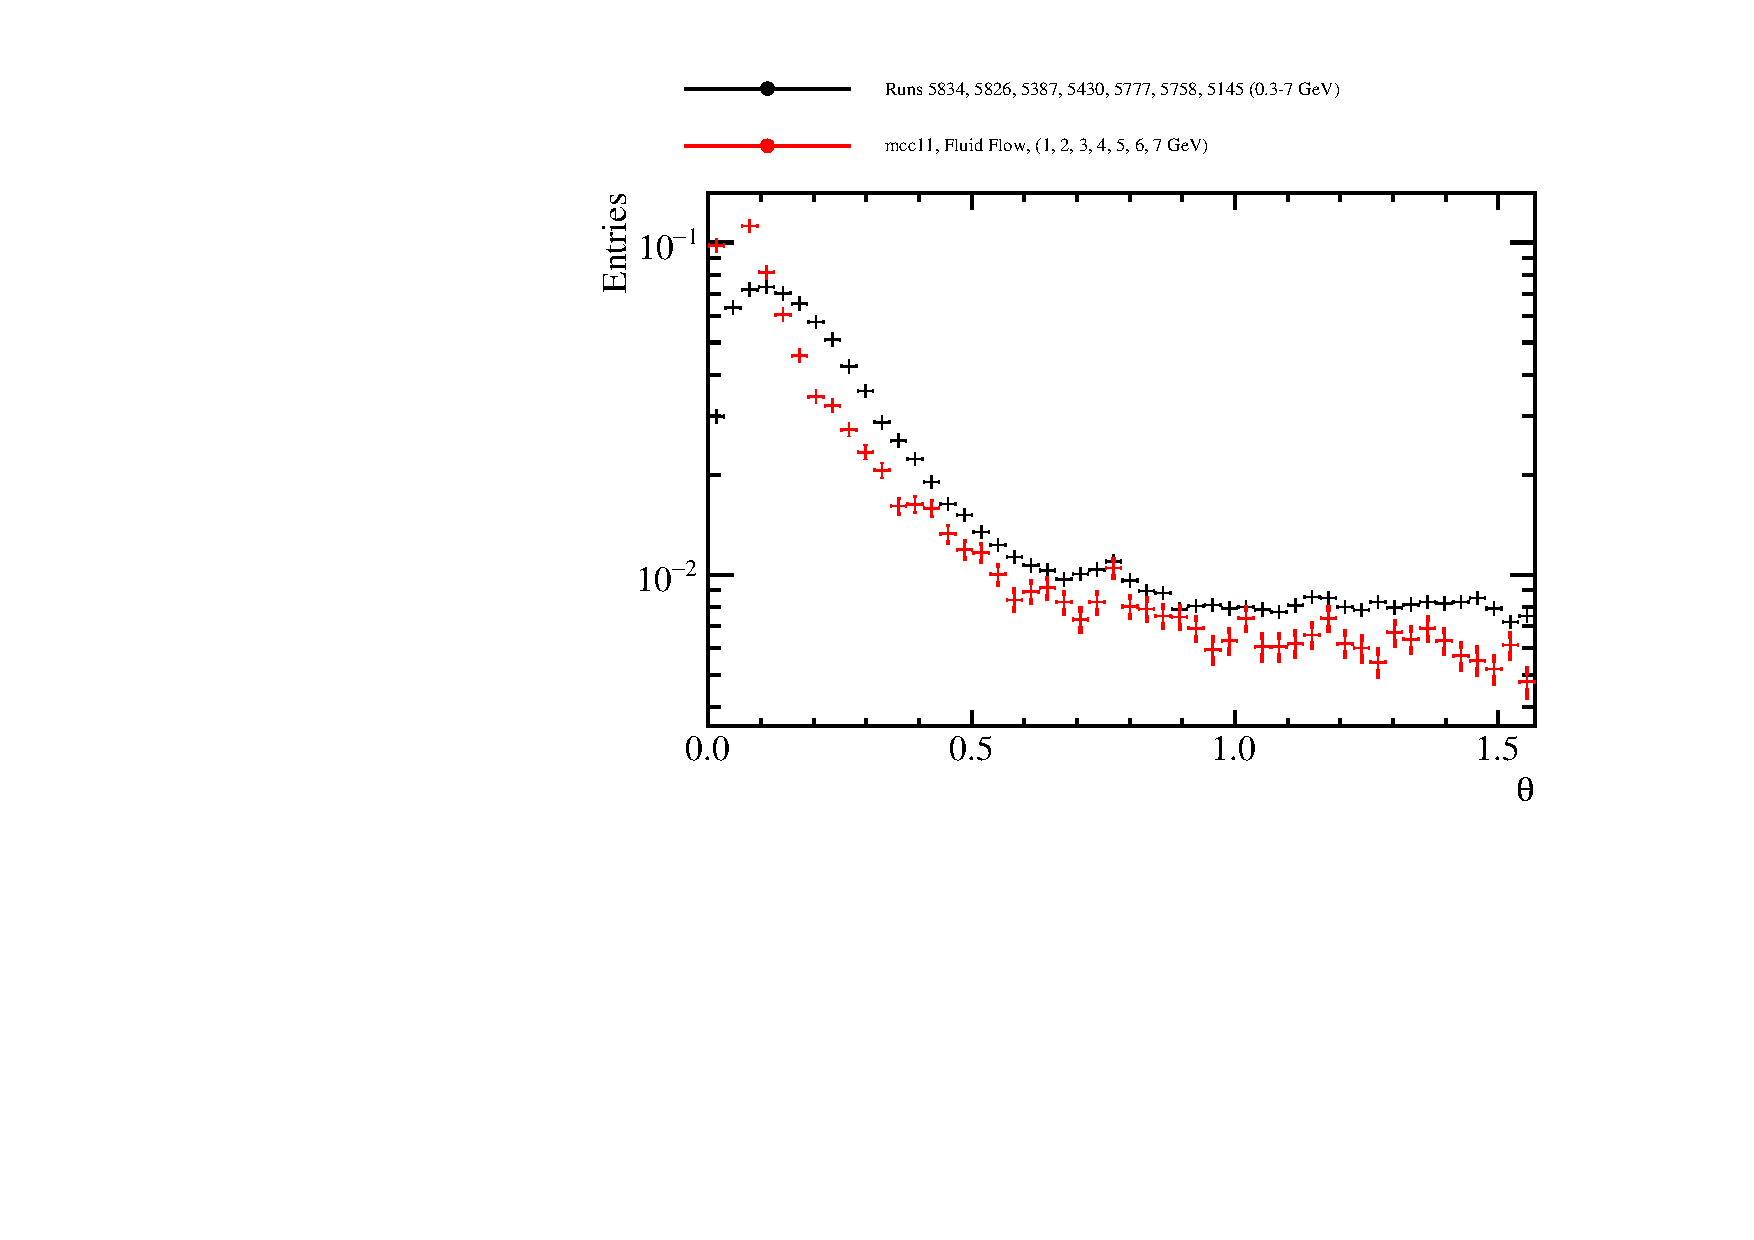
\includegraphics[width=1.0\textwidth]{Figures/Metrics/Data/Beam/BeamParticleOpeningAngle.pdf}
\caption{The opening angle between a linear fit to the start of the reconstructed test beam particle as it enters the TPC and the MC truth direction direction.}
\label{fig:8}
\end{figure}

\subsubsection{Cosmic Ray Metrics}

Lorem ipsum dolor sit amet, consectetur adipiscing elit. Duis consectetur neque vel urna accumsan, sed tincidunt sapien tincidunt. Aenean imperdiet vitae odio rhoncus sollicitudin. Praesent nec vehicula ante. Cras aliquam hendrerit lectus, nec rutrum urna tempor a. Aliquam sit amet mattis nisl. Nam molestie a elit consectetur auctor. Lorem ipsum dolor sit amet, consectetur adipiscing elit. Nam ac magna id turpis euismod accumsan.

\begin{figure}
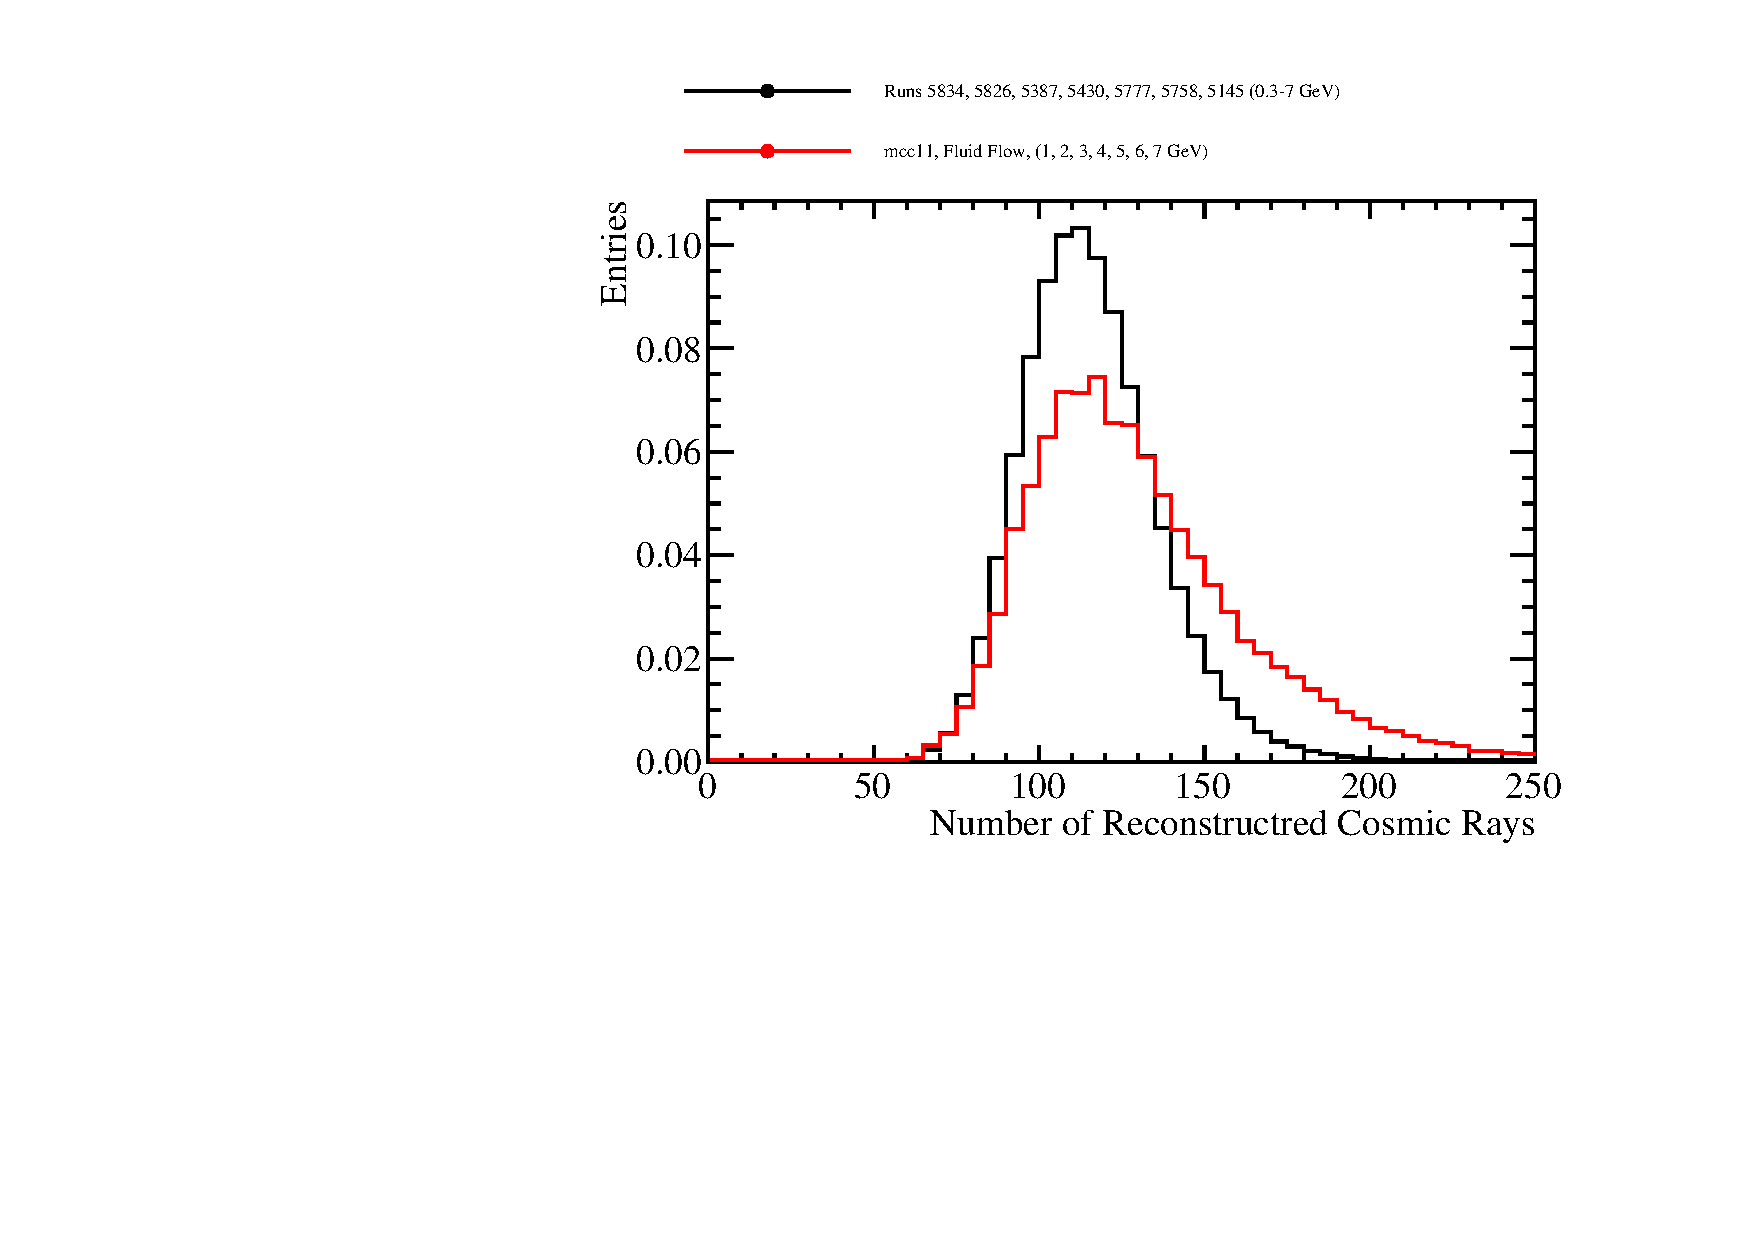
\includegraphics[width=1.0\textwidth]{Figures/Metrics/Data/Cosmics/NumberofReconstructedCosmicRays.pdf}
\caption{Please write your figure caption here}
\label{fig:9}
\end{figure}

\begin{figure}
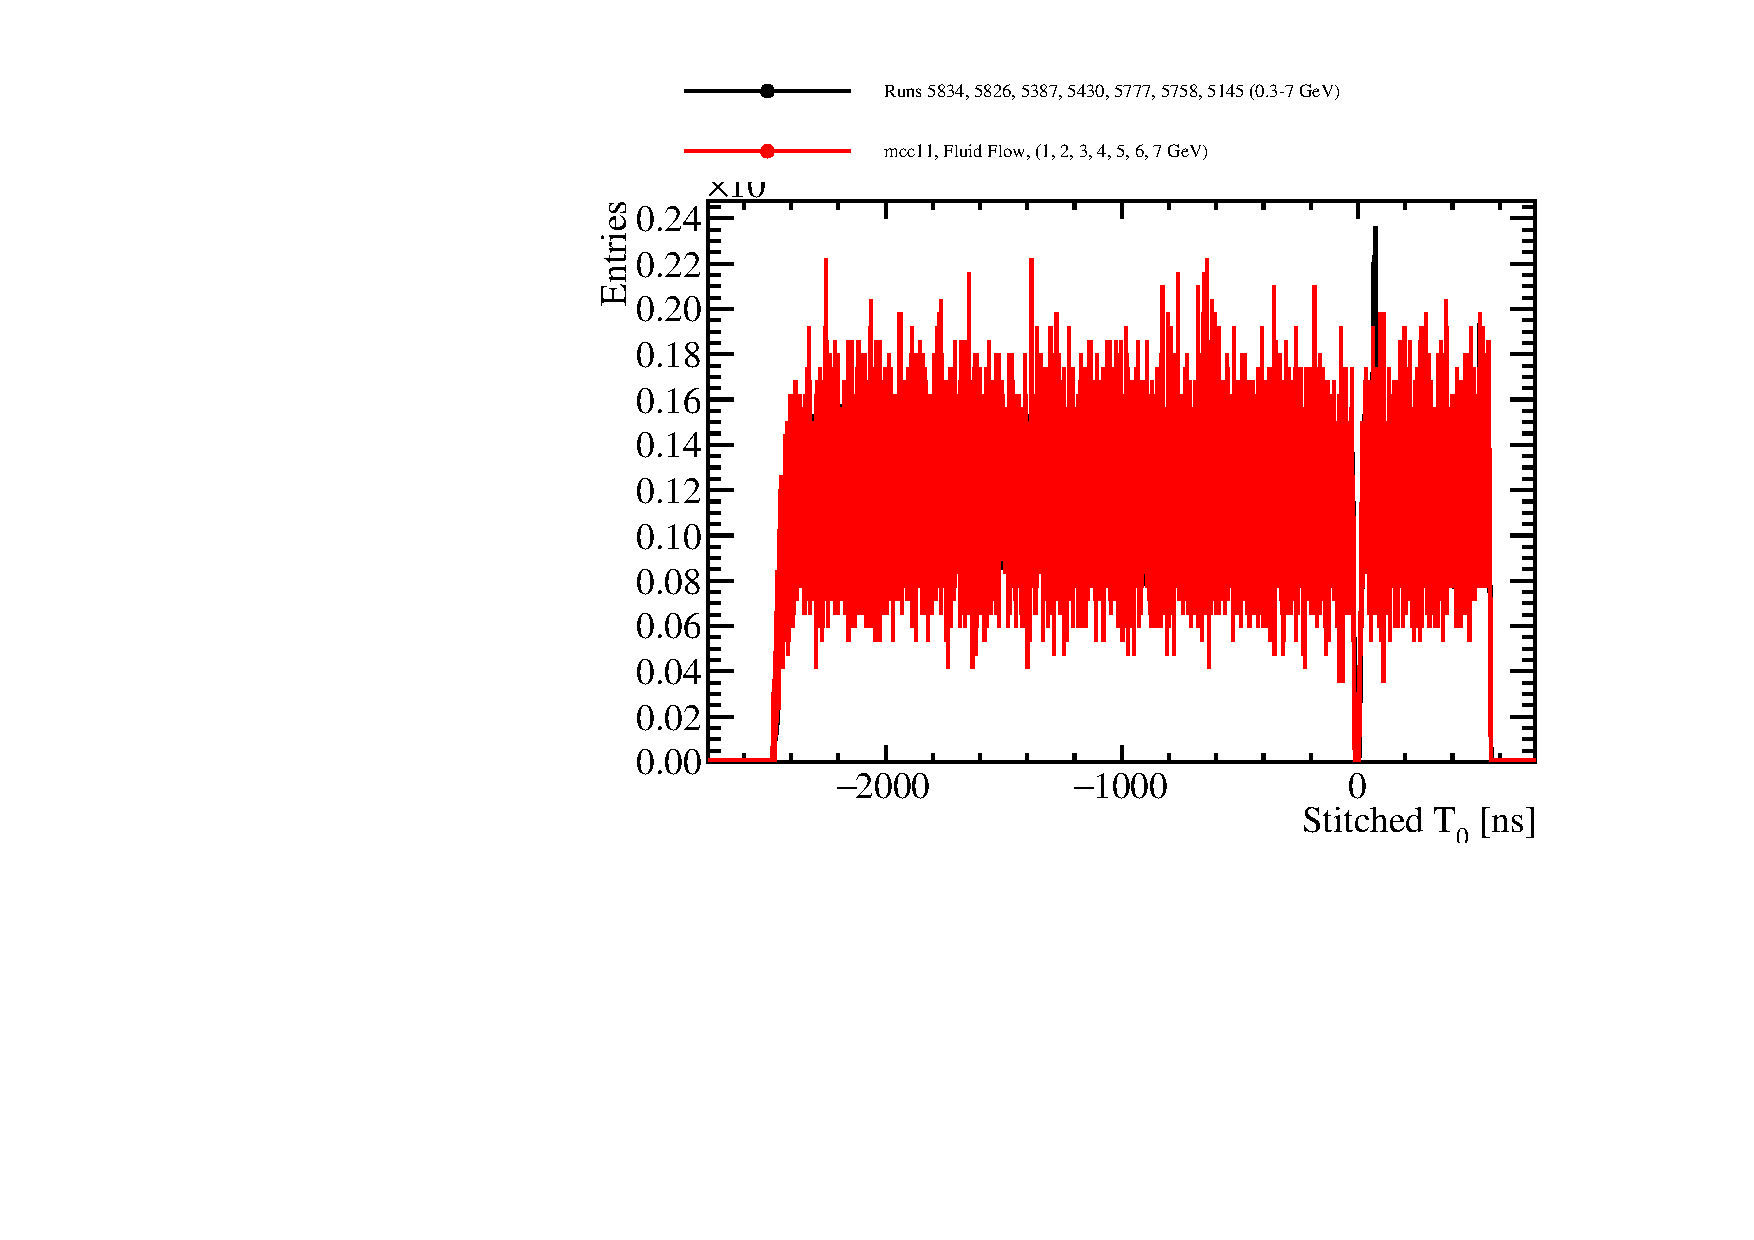
\includegraphics[width=1.0\textwidth]{Figures/Metrics/Data/Cosmics/StitchedT0.pdf}
\caption{Please write your figure caption here}
\label{fig:10}
\end{figure}

\section{Conclusions}

Lorem ipsum dolor sit amet, consectetur adipiscing elit. Duis consectetur neque vel urna accumsan, sed tincidunt sapien tincidunt. Aenean imperdiet vitae odio rhoncus sollicitudin. Praesent nec vehicula ante. Cras aliquam hendrerit lectus, nec rutrum urna tempor a. Aliquam sit amet mattis nisl. Nam molestie a elit consectetur auctor. Lorem ipsum dolor sit amet, consectetur adipiscing elit. Nam ac magna id turpis euismod accumsan.

Aliquam gravida urna a arcu euismod, eget ultricies enim placerat. Vestibulum ultrices ultricies eleifend. Proin vestibulum risus eu ultrices condimentum. Interdum et malesuada fames ac ante ipsum primis in faucibus. Aliquam id urna in dui tristique feugiat. Nullam in dui diam. Etiam sit amet eros vel mi egestas scelerisque sed nec nibh. Vivamus imperdiet risus sed quam commodo vehicula. Nulla in arcu scelerisque, luctus urna ut, ullamcorper est. Fusce tristique eros in tempus egestas. Phasellus non mattis risus. Quisque sed tristique lectus. Donec porttitor commodo enim dictum facilisis.

Pellentesque consequat accumsan auctor. Vivamus efficitur urna a augue molestie lacinia. Morbi et facilisis quam. Praesent libero velit, lobortis ac posuere sit amet, pharetra non nunc. Donec porttitor malesuada tristique. Suspendisse suscipit ultrices turpis, congue mattis odio facilisis ac. Proin ornare metus a velit lacinia, non vulputate massa ultrices. Proin diam leo, tristique non lectus ut, pellentesque malesuada enim. Phasellus tortor nulla, cursus ac sapien in, tempor sollicitudin ante. Ut ac dui nec erat eleifend varius. Vestibulum placerat urna quis feugiat imperdiet.

%\begin{acknowledgements}
%If you'd like to thank anyone, place your comments here
%and remove the percent signs.
%\end{acknowledgements}

% BibTeX users please use one of
%\bibliographystyle{spbasic}      % basic style, author-year citations
%\bibliographystyle{spmpsci}      % mathematics and physical sciences
%\bibliographystyle{spphys}       % APS-like style for physics
%\bibliography{}   % name your BibTeX data base

% Non-BibTeX users please use
\begin{thebibliography}{}
%
% and use \bibitem to create references. Consult the Instructions
% for authors for reference list style.
%
\bibitem{RefJ}
% Format for Journal Reference
Author, Article title, Journal, Volume, page numbers (year)
% Format for books
\bibitem{RefB}
Author, Book title, page numbers. Publisher, place (year)
% etc
\end{thebibliography}

\end{document}
% end of file template.tex

